% CasePath: An Agentic, Process-First Architecture for Determining Evidence Requirements
% ICLR 2027 submission. The submitted title and abstract are preserved verbatim.
% All numbers are macros generated from preserved evidence (evidence/build_manuscript_numbers.py).
\documentclass{article}
\usepackage[T1]{fontenc}
\ifdefined\XeTeXversion
\usepackage{newunicodechar}
\newunicodechar{—}{\textemdash}
\fi
\usepackage{iclr2027_conference,times}
\input{math_commands.tex}
\usepackage{hyperref,url,booktabs,amsmath,amssymb,graphicx,microtype,xurl,xcolor,array,xspace,placeins,tabularx}
\hypersetup{colorlinks=true,linkcolor=black,citecolor=black,urlcolor=black}
\newcommand{\casepath}{\textsc{CasePath}\xspace}
\newcommand{\T}{\mathsf{T}}
\newcommand{\F}{\mathsf{F}}
\newcommand{\U}{\mathsf{U}}
% GENERATED by evidence/build_manuscript_numbers.py -- do not edit by hand.
\newcommand{\nGoldAtoms}{33}
\newcommand{\nPairsHid}{27}
\newcommand{\cpPrec}{0.615}
\newcommand{\cpRec}{0.727}
\newcommand{\cpF}{0.667}
\newcommand{\cpExact}{0.444}
\newcommand{\cpExactN}{12}
\newcommand{\cpPred}{39}
\newcommand{\cpTP}{24}
\newcommand{\cpSpur}{15}
\newcommand{\cpMiss}{9}
\newcommand{\cpRatio}{1.18}
\newcommand{\cpMacro}{0.648}
\newcommand{\cpCIlo}{0.435}
\newcommand{\cpCIhi}{0.880}
\newcommand{\dirPrec}{0.481}
\newcommand{\dirRec}{0.758}
\newcommand{\dirF}{0.588}
\newcommand{\dirExact}{0.333}
\newcommand{\dirExactN}{9}
\newcommand{\dirPred}{52}
\newcommand{\dirTP}{25}
\newcommand{\dirSpur}{27}
\newcommand{\dirMiss}{8}
\newcommand{\dirRatio}{1.58}
\newcommand{\dirMacro}{0.612}
\newcommand{\dirCIlo}{0.404}
\newcommand{\dirCIhi}{0.759}
\newcommand{\gcPrec}{0.431}
\newcommand{\gcRec}{0.939}
\newcommand{\gcF}{0.590}
\newcommand{\gcExact}{0.148}
\newcommand{\gcExactN}{4}
\newcommand{\gcPred}{72}
\newcommand{\gcTP}{31}
\newcommand{\gcSpur}{41}
\newcommand{\gcMiss}{2}
\newcommand{\gcRatio}{2.18}
\newcommand{\gcMacro}{0.605}
\newcommand{\gcCIlo}{0.471}
\newcommand{\gcCIhi}{0.716}
\newcommand{\efPrec}{0.235}
\newcommand{\efRec}{0.485}
\newcommand{\efF}{0.317}
\newcommand{\efExact}{0.074}
\newcommand{\efExactN}{2}
\newcommand{\efPred}{68}
\newcommand{\efTP}{16}
\newcommand{\efSpur}{52}
\newcommand{\efMiss}{17}
\newcommand{\efRatio}{2.06}
\newcommand{\efMacro}{0.314}
\newcommand{\efCIlo}{0.239}
\newcommand{\efCIhi}{0.400}
\newcommand{\dDirLo}{-0.253}
\newcommand{\dDirHi}{+0.420}
\newcommand{\mDir}{+0.078}
\newcommand{\pHolmDir}{0.797}
\newcommand{\pRawDir}{0.436}
\newcommand{\redDir}{44.4}
\newcommand{\dGcLo}{-0.199}
\newcommand{\dGcHi}{+0.333}
\newcommand{\mGc}{+0.076}
\newcommand{\pHolmGc}{0.797}
\newcommand{\pRawGc}{0.398}
\newcommand{\redGc}{63.4}
\newcommand{\dEfLo}{+0.110}
\newcommand{\dEfHi}{+0.565}
\newcommand{\mEf}{+0.350}
\newcommand{\pHolmEf}{0.129}
\newcommand{\pRawEf}{0.043}
\newcommand{\redEf}{71.2}
\newcommand{\wpObs}{0.667}
\newcommand{\wpMax}{0.083}
\newcommand{\wpNinetySevenFive}{0.083}
\newcommand{\wpMean}{0.011}
\newcommand{\wpP}{1.996\times10^{-4}}
\newcommand{\wpDraws}{5,000}
\newcommand{\wpShifts}{8}
\newcommand{\wpEvaluated}{5,008}
\newcommand{\chainAttributed}{39}
\newcommand{\chainPredicted}{39}
\newcommand{\chainCovered}{27}
\newcommand{\chainCoverage}{81.8}
\newcommand{\bootDraws}{10,000}
\newcommand{\bootSeed}{20260917}
\newcommand{\swapAssignments}{512}
\newcommand{\ratioAll}{1.18}
\newcommand{\pfNoInputMax}{0.0}
\newcommand{\pfSignatures}{9}
\newcommand{\pfEntropy}{3.17}
\newcommand{\nPairsAll}{36}
\newcommand{\nUnitsAll}{72}
\newcommand{\nConcepts}{9}
\newcommand{\pfUniverse}{12}
\newcommand{\nPassages}{197}
\newcommand{\nPropositions}{308}
\newcommand{\nRules}{98}
\newcommand{\nGuards}{87}
\newcommand{\nNonEvidentiary}{13}
\newcommand{\nCatalogue}{33}
\newcommand{\nPairsDev}{9}
\newcommand{\nUnitsDev}{18}
\newcommand{\nUnitsHid}{54}
\newcommand{\cpCalls}{87}
\newcommand{\cpCost}{5.44}
\newcommand{\cpPromptTok}{1.01M}
\newcommand{\cpComplTok}{243.9k}
\newcommand{\cpMaxTok}{10,000}
\newcommand{\cpModel}{openai/gpt-5.6-terra}
\newcommand{\dirCalls}{54}
\newcommand{\dirCost}{4.83}
\newcommand{\dirPromptTok}{2.90M}
\newcommand{\dirComplTok}{45.7k}
\newcommand{\dirMaxTok}{14,000}
\newcommand{\dirModel}{openai/gpt-5.6-terra}
\newcommand{\gcCalls}{54}
\newcommand{\gcCost}{8.41}
\newcommand{\gcPromptTok}{5.35M}
\newcommand{\gcComplTok}{42.7k}
\newcommand{\gcMaxTok}{14,000}
\newcommand{\gcModel}{openai/gpt-5.6-terra}
\newcommand{\efCalls}{108}
\newcommand{\efCost}{1.06}
\newcommand{\efPromptTok}{0.26M}
\newcommand{\efComplTok}{66.5k}
\newcommand{\efMaxTok}{14,000/18,000}
\newcommand{\efModel}{openai/gpt-5.6-terra}
\newcommand{\parityUnits}{72}
\newcommand{\parityPairs}{36}
\newcommand{\parityAllMatch}{all}
\newcommand{\nbClaims}{150}
\newcommand{\nbFamilies}{28}
\newcommand{\nbCells}{1,050}
\newcommand{\nbLearnedCells}{750}
\newcommand{\nbDependentCells}{300}
\newcommand{\nbDevClaims}{60}
\newcommand{\nbDevFamilies}{11}
\newcommand{\nbDevCells}{420}
\newcommand{\nbHidClaims}{90}
\newcommand{\nbHidFamilies}{17}
\newcommand{\nbHidCells}{630}
\newcommand{\nbTokens}{4,096}
\newcommand{\nbCallsPerCell}{2}
\newcommand{\nbModel}{openai/gpt-5.6-terra}
\newcommand{\nbReasoning}{medium}
\newcommand{\nbLearnedArms}{5}
\newcommand{\nbDependentArms}{2}
\newcommand{\nbRecorded}{829}
\newcommand{\nbDevRecorded}{420}
\newcommand{\nbHidRecorded}{409}
\newcommand{\bCpDevOk}{44}
\newcommand{\bCpDevFail}{16}
\newcommand{\bCpDevBlocked}{0}
\newcommand{\bCpDevEndpoint}{0}
\newcommand{\bCpDevTrunc}{2}
\newcommand{\bCpDevCodebook}{4}
\newcommand{\bCpDevPresence}{7}
\newcommand{\bDirDevOk}{19}
\newcommand{\bDirDevFail}{41}
\newcommand{\bDirDevBlocked}{0}
\newcommand{\bDirDevEndpoint}{21}
\newcommand{\bDirDevTrunc}{10}
\newcommand{\bDirDevCodebook}{8}
\newcommand{\bDirDevPresence}{0}
\newcommand{\bDocDevOk}{17}
\newcommand{\bDocDevFail}{43}
\newcommand{\bDocDevBlocked}{0}
\newcommand{\bDocDevEndpoint}{13}
\newcommand{\bDocDevTrunc}{16}
\newcommand{\bDocDevCodebook}{11}
\newcommand{\bDocDevPresence}{0}
\newcommand{\bPcDevOk}{27}
\newcommand{\bPcDevFail}{33}
\newcommand{\bPcDevBlocked}{0}
\newcommand{\bPcDevEndpoint}{26}
\newcommand{\bPcDevTrunc}{5}
\newcommand{\bPcDevCodebook}{1}
\newcommand{\bPcDevPresence}{0}
\newcommand{\bRfDevOk}{28}
\newcommand{\bRfDevFail}{32}
\newcommand{\bRfDevBlocked}{0}
\newcommand{\bRfDevEndpoint}{21}
\newcommand{\bRfDevTrunc}{8}
\newcommand{\bRfDevCodebook}{3}
\newcommand{\bRfDevPresence}{0}
\newcommand{\bCeDevOk}{44}
\newcommand{\bCeDevFail}{0}
\newcommand{\bCeDevBlocked}{16}
\newcommand{\bCeDevEndpoint}{0}
\newcommand{\bCeDevTrunc}{0}
\newcommand{\bCeDevCodebook}{0}
\newcommand{\bCeDevPresence}{0}
\newcommand{\bLsDevOk}{44}
\newcommand{\bLsDevFail}{0}
\newcommand{\bLsDevBlocked}{16}
\newcommand{\bLsDevEndpoint}{0}
\newcommand{\bLsDevTrunc}{0}
\newcommand{\bLsDevCodebook}{0}
\newcommand{\bLsDevPresence}{0}
\newcommand{\cpFamScheduled}{0.667}
\newcommand{\cpFamSim}{0.667}
\newcommand{\cpFamRepair}{0.500}
\newcommand{\gateMargin}{0.10}
\newcommand{\gatePrec}{0.70}
\newcommand{\bndF}{+0.03}
\newcommand{\bndCer}{-0.03}
\newcommand{\bndUdr}{-0.03}
\newcommand{\nbPrimaryContrasts}{12}
\newcommand{\efMaxTokExtract}{18,000}
\newcommand{\efMaxTokPlan}{14,000}
\newcommand{\cpMaxTokGuard}{10,000}
\newcommand{\dirMaxTokCall}{14,000}
\newcommand{\pairExampleFalse}{No stolen item is separately scheduled in the policy with an insured value of CHF 1,000 or more}
\newcommand{\pairExampleTrue}{A stolen watch is separately scheduled in the policy with an insured value of CHF 4,000}

% Generated from authenticated native150 evidence.
\newcommand{\rqDevCpN}{44}
\newcommand{\rqDevCpP}{0.704}
\newcommand{\rqDevCpR}{0.635}
\newcommand{\rqDevCpF}{0.657}
\newcommand{\rqDevCpExact}{0.247}
\newcommand{\rqDevCpU}{0.296}
\newcommand{\rqDevCpCorrect}{259}
\newcommand{\rqDevCpRequested}{275}
\newcommand{\rqDevCpMissed}{41}
\newcommand{\rqDevCpExtra}{16}
\newcommand{\rqDevCpRequired}{300}
\newcommand{\rqDevCpConditional}{811}
\newcommand{\rqDevDirN}{19}
\newcommand{\rqDevDirP}{0.313}
\newcommand{\rqDevDirR}{0.281}
\newcommand{\rqDevDirF}{0.295}
\newcommand{\rqDevDirExact}{0.116}
\newcommand{\rqDevDirU}{0.687}
\newcommand{\rqDevDirCorrect}{114}
\newcommand{\rqDevDirRequested}{116}
\newcommand{\rqDevDirMissed}{16}
\newcommand{\rqDevDirExtra}{2}
\newcommand{\rqDevDirRequired}{130}
\newcommand{\rqDevDirConditional}{23}
\newcommand{\rqDevDocN}{17}
\newcommand{\rqDevDocP}{0.268}
\newcommand{\rqDevDocR}{0.233}
\newcommand{\rqDevDocF}{0.247}
\newcommand{\rqDevDocExact}{0.049}
\newcommand{\rqDevDocU}{0.732}
\newcommand{\rqDevDocCorrect}{95}
\newcommand{\rqDevDocRequested}{103}
\newcommand{\rqDevDocMissed}{22}
\newcommand{\rqDevDocExtra}{8}
\newcommand{\rqDevDocRequired}{117}
\newcommand{\rqDevDocConditional}{84}
\newcommand{\rqDevPcN}{27}
\newcommand{\rqDevPcP}{0.430}
\newcommand{\rqDevPcR}{0.394}
\newcommand{\rqDevPcF}{0.407}
\newcommand{\rqDevPcExact}{0.166}
\newcommand{\rqDevPcU}{0.570}
\newcommand{\rqDevPcCorrect}{163}
\newcommand{\rqDevPcRequested}{169}
\newcommand{\rqDevPcMissed}{23}
\newcommand{\rqDevPcExtra}{6}
\newcommand{\rqDevPcRequired}{186}
\newcommand{\rqDevPcConditional}{15}
\newcommand{\rqDevRfN}{28}
\newcommand{\rqDevRfP}{0.455}
\newcommand{\rqDevRfR}{0.414}
\newcommand{\rqDevRfF}{0.433}
\newcommand{\rqDevRfExact}{0.197}
\newcommand{\rqDevRfU}{0.545}
\newcommand{\rqDevRfCorrect}{171}
\newcommand{\rqDevRfRequested}{174}
\newcommand{\rqDevRfMissed}{21}
\newcommand{\rqDevRfExtra}{3}
\newcommand{\rqDevRfRequired}{192}
\newcommand{\rqDevRfConditional}{11}
\newcommand{\rqDevCeN}{44}
\newcommand{\rqDevCeP}{0.704}
\newcommand{\rqDevCeR}{0.635}
\newcommand{\rqDevCeF}{0.657}
\newcommand{\rqDevCeExact}{0.247}
\newcommand{\rqDevCeU}{0.296}
\newcommand{\rqDevCeCorrect}{259}
\newcommand{\rqDevCeRequested}{275}
\newcommand{\rqDevCeMissed}{41}
\newcommand{\rqDevCeExtra}{16}
\newcommand{\rqDevCeRequired}{300}
\newcommand{\rqDevCeConditional}{811}
\newcommand{\rqDevLsN}{44}
\newcommand{\rqDevLsP}{0.331}
\newcommand{\rqDevLsR}{0.635}
\newcommand{\rqDevLsF}{0.420}
\newcommand{\rqDevLsExact}{0.000}
\newcommand{\rqDevLsU}{0.669}
\newcommand{\rqDevLsCorrect}{259}
\newcommand{\rqDevLsRequested}{592}
\newcommand{\rqDevLsMissed}{41}
\newcommand{\rqDevLsExtra}{333}
\newcommand{\rqDevLsRequired}{300}
\newcommand{\rqDevLsConditional}{560}
\newcommand{\rqDevDDirP}{+0.392}
\newcommand{\rqDevCDirP}{-0.772}
\newcommand{\rqDevDDirR}{+0.354}
\newcommand{\rqDevCDirR}{-0.767}
\newcommand{\rqDevDDirF}{+0.361}
\newcommand{\rqDevCDirF}{-0.770}
\newcommand{\rqDevDDirExact}{+0.131}
\newcommand{\rqDevCDirExact}{-0.765}
\newcommand{\rqDevDDirU}{+0.392}
\newcommand{\rqDevCDirU}{-0.772}
\newcommand{\rqDevDDocP}{+0.436}
\newcommand{\rqDevCDocP}{-0.787}
\newcommand{\rqDevDDocR}{+0.402}
\newcommand{\rqDevCDocR}{-0.784}
\newcommand{\rqDevDDocF}{+0.410}
\newcommand{\rqDevCDocF}{-0.786}
\newcommand{\rqDevDDocExact}{+0.198}
\newcommand{\rqDevCDocExact}{-0.795}
\newcommand{\rqDevDDocU}{+0.436}
\newcommand{\rqDevCDocU}{-0.787}
\newcommand{\rqDevDPcP}{+0.274}
\newcommand{\rqDevCPcP}{-0.632}
\newcommand{\rqDevDPcR}{+0.241}
\newcommand{\rqDevCPcR}{-0.647}
\newcommand{\rqDevDPcF}{+0.249}
\newcommand{\rqDevCPcF}{-0.646}
\newcommand{\rqDevDPcExact}{+0.081}
\newcommand{\rqDevCPcExact}{-0.635}
\newcommand{\rqDevDPcU}{+0.274}
\newcommand{\rqDevCPcU}{-0.632}
\newcommand{\rqDevDRfP}{+0.249}
\newcommand{\rqDevCRfP}{-0.640}
\newcommand{\rqDevDRfR}{+0.221}
\newcommand{\rqDevCRfR}{-0.639}
\newcommand{\rqDevDRfF}{+0.224}
\newcommand{\rqDevCRfF}{-0.640}
\newcommand{\rqDevDRfExact}{+0.050}
\newcommand{\rqDevCRfExact}{-0.651}
\newcommand{\rqDevDRfU}{+0.249}
\newcommand{\rqDevCRfU}{-0.640}
\newcommand{\rqHidCpN}{66}
\newcommand{\rqHidCpP}{0.732}
\newcommand{\rqHidCpR}{0.645}
\newcommand{\rqHidCpF}{0.677}
\newcommand{\rqHidCpExact}{0.333}
\newcommand{\rqHidCpU}{0.268}
\newcommand{\rqHidCpCorrect}{384}
\newcommand{\rqHidCpRequested}{385}
\newcommand{\rqHidCpMissed}{54}
\newcommand{\rqHidCpExtra}{1}
\newcommand{\rqHidCpRequired}{438}
\newcommand{\rqHidCpConditional}{1195}
\newcommand{\rqHidDirN}{30}
\newcommand{\rqHidDirP}{0.312}
\newcommand{\rqHidDirR}{0.310}
\newcommand{\rqHidDirF}{0.310}
\newcommand{\rqHidDirExact}{0.156}
\newcommand{\rqHidDirU}{0.688}
\newcommand{\rqHidDirCorrect}{187}
\newcommand{\rqHidDirRequested}{200}
\newcommand{\rqHidDirMissed}{14}
\newcommand{\rqHidDirExtra}{13}
\newcommand{\rqHidDirRequired}{201}
\newcommand{\rqHidDirConditional}{42}
\newcommand{\rqHidDocN}{24}
\newcommand{\rqHidDocP}{0.263}
\newcommand{\rqHidDocR}{0.238}
\newcommand{\rqHidDocF}{0.249}
\newcommand{\rqHidDocExact}{0.144}
\newcommand{\rqHidDocU}{0.737}
\newcommand{\rqHidDocCorrect}{142}
\newcommand{\rqHidDocRequested}{144}
\newcommand{\rqHidDocMissed}{17}
\newcommand{\rqHidDocExtra}{2}
\newcommand{\rqHidDocRequired}{159}
\newcommand{\rqHidDocConditional}{55}
\newcommand{\rqHidPcN}{43}
\newcommand{\rqHidPcP}{0.462}
\newcommand{\rqHidPcR}{0.456}
\newcommand{\rqHidPcF}{0.458}
\newcommand{\rqHidPcExact}{0.278}
\newcommand{\rqHidPcU}{0.538}
\newcommand{\rqHidPcCorrect}{270}
\newcommand{\rqHidPcRequested}{280}
\newcommand{\rqHidPcMissed}{13}
\newcommand{\rqHidPcExtra}{10}
\newcommand{\rqHidPcRequired}{283}
\newcommand{\rqHidPcConditional}{16}
\newcommand{\rqHidRfN}{42}
\newcommand{\rqHidRfP}{0.460}
\newcommand{\rqHidRfR}{0.443}
\newcommand{\rqHidRfF}{0.450}
\newcommand{\rqHidRfExact}{0.311}
\newcommand{\rqHidRfU}{0.540}
\newcommand{\rqHidRfCorrect}{261}
\newcommand{\rqHidRfRequested}{265}
\newcommand{\rqHidRfMissed}{15}
\newcommand{\rqHidRfExtra}{4}
\newcommand{\rqHidRfRequired}{276}
\newcommand{\rqHidRfConditional}{25}
\newcommand{\rqHidCeN}{66}
\newcommand{\rqHidCeP}{0.732}
\newcommand{\rqHidCeR}{0.645}
\newcommand{\rqHidCeF}{0.677}
\newcommand{\rqHidCeExact}{0.333}
\newcommand{\rqHidCeU}{0.268}
\newcommand{\rqHidCeCorrect}{384}
\newcommand{\rqHidCeRequested}{385}
\newcommand{\rqHidCeMissed}{54}
\newcommand{\rqHidCeExtra}{1}
\newcommand{\rqHidCeRequired}{438}
\newcommand{\rqHidCeConditional}{1195}
\newcommand{\rqHidLsN}{64}
\newcommand{\rqHidLsP}{0.318}
\newcommand{\rqHidLsR}{0.627}
\newcommand{\rqHidLsF}{0.411}
\newcommand{\rqHidLsExact}{0.000}
\newcommand{\rqHidLsU}{0.682}
\newcommand{\rqHidLsCorrect}{376}
\newcommand{\rqHidLsRequested}{853}
\newcommand{\rqHidLsMissed}{52}
\newcommand{\rqHidLsExtra}{477}
\newcommand{\rqHidLsRequired}{428}
\newcommand{\rqHidLsConditional}{827}
\newcommand{\rqHidDDirP}{+0.419}
\newcommand{\rqHidCDirP}{-0.744}
\newcommand{\rqHidDDirR}{+0.335}
\newcommand{\rqHidCDirR}{-0.769}
\newcommand{\rqHidDDirF}{+0.367}
\newcommand{\rqHidCDirF}{-0.758}
\newcommand{\rqHidDDirExact}{+0.178}
\newcommand{\rqHidCDirExact}{-0.822}
\newcommand{\rqHidDDirU}{+0.419}
\newcommand{\rqHidCDirU}{-0.744}
\newcommand{\rqHidDDocP}{+0.469}
\newcommand{\rqHidCDocP}{-0.785}
\newcommand{\rqHidDDocR}{+0.406}
\newcommand{\rqHidCDocR}{-0.790}
\newcommand{\rqHidDDocF}{+0.429}
\newcommand{\rqHidCDocF}{-0.788}
\newcommand{\rqHidDDocExact}{+0.189}
\newcommand{\rqHidCDocExact}{-0.789}
\newcommand{\rqHidDDocU}{+0.469}
\newcommand{\rqHidCDocU}{-0.785}
\newcommand{\rqHidDPcP}{+0.270}
\newcommand{\rqHidCPcP}{-0.657}
\newcommand{\rqHidDPcR}{+0.189}
\newcommand{\rqHidCPcR}{-0.686}
\newcommand{\rqHidDPcF}{+0.219}
\newcommand{\rqHidCPcF}{-0.673}
\newcommand{\rqHidDPcExact}{+0.056}
\newcommand{\rqHidCPcExact}{-0.711}
\newcommand{\rqHidDPcU}{+0.270}
\newcommand{\rqHidCPcU}{-0.657}
\newcommand{\rqHidDRfP}{+0.272}
\newcommand{\rqHidCRfP}{-0.650}
\newcommand{\rqHidDRfR}{+0.202}
\newcommand{\rqHidCRfR}{-0.679}
\newcommand{\rqHidDRfF}{+0.227}
\newcommand{\rqHidCRfF}{-0.671}
\newcommand{\rqHidDRfExact}{+0.022}
\newcommand{\rqHidCRfExact}{-0.711}
\newcommand{\rqHidDRfU}{+0.272}
\newcommand{\rqHidCRfU}{-0.650}
\newcommand{\rqAllCpN}{110}
\newcommand{\rqAllCpP}{0.721}
\newcommand{\rqAllCpR}{0.641}
\newcommand{\rqAllCpF}{0.669}
\newcommand{\rqAllCpExact}{0.300}
\newcommand{\rqAllCpU}{0.279}
\newcommand{\rqAllCpCorrect}{643}
\newcommand{\rqAllCpRequested}{660}
\newcommand{\rqAllCpMissed}{95}
\newcommand{\rqAllCpExtra}{17}
\newcommand{\rqAllCpRequired}{738}
\newcommand{\rqAllCpConditional}{2006}
\newcommand{\rqAllDirN}{49}
\newcommand{\rqAllDirP}{0.312}
\newcommand{\rqAllDirR}{0.298}
\newcommand{\rqAllDirF}{0.304}
\newcommand{\rqAllDirExact}{0.140}
\newcommand{\rqAllDirU}{0.688}
\newcommand{\rqAllDirCorrect}{301}
\newcommand{\rqAllDirRequested}{316}
\newcommand{\rqAllDirMissed}{30}
\newcommand{\rqAllDirExtra}{15}
\newcommand{\rqAllDirRequired}{331}
\newcommand{\rqAllDirConditional}{65}
\newcommand{\rqAllDocN}{41}
\newcommand{\rqAllDocP}{0.265}
\newcommand{\rqAllDocR}{0.236}
\newcommand{\rqAllDocF}{0.248}
\newcommand{\rqAllDocExact}{0.107}
\newcommand{\rqAllDocU}{0.735}
\newcommand{\rqAllDocCorrect}{237}
\newcommand{\rqAllDocRequested}{247}
\newcommand{\rqAllDocMissed}{39}
\newcommand{\rqAllDocExtra}{10}
\newcommand{\rqAllDocRequired}{276}
\newcommand{\rqAllDocConditional}{139}
\newcommand{\rqAllPcN}{70}
\newcommand{\rqAllPcP}{0.451}
\newcommand{\rqAllPcR}{0.434}
\newcommand{\rqAllPcF}{0.440}
\newcommand{\rqAllPcExact}{0.236}
\newcommand{\rqAllPcU}{0.549}
\newcommand{\rqAllPcCorrect}{433}
\newcommand{\rqAllPcRequested}{449}
\newcommand{\rqAllPcMissed}{36}
\newcommand{\rqAllPcExtra}{16}
\newcommand{\rqAllPcRequired}{469}
\newcommand{\rqAllPcConditional}{31}
\newcommand{\rqAllRfN}{70}
\newcommand{\rqAllRfP}{0.458}
\newcommand{\rqAllRfR}{0.432}
\newcommand{\rqAllRfF}{0.443}
\newcommand{\rqAllRfExact}{0.266}
\newcommand{\rqAllRfU}{0.542}
\newcommand{\rqAllRfCorrect}{432}
\newcommand{\rqAllRfRequested}{439}
\newcommand{\rqAllRfMissed}{36}
\newcommand{\rqAllRfExtra}{7}
\newcommand{\rqAllRfRequired}{468}
\newcommand{\rqAllRfConditional}{36}
\newcommand{\rqAllCeN}{110}
\newcommand{\rqAllCeP}{0.721}
\newcommand{\rqAllCeR}{0.641}
\newcommand{\rqAllCeF}{0.669}
\newcommand{\rqAllCeExact}{0.300}
\newcommand{\rqAllCeU}{0.279}
\newcommand{\rqAllCeCorrect}{643}
\newcommand{\rqAllCeRequested}{660}
\newcommand{\rqAllCeMissed}{95}
\newcommand{\rqAllCeExtra}{17}
\newcommand{\rqAllCeRequired}{738}
\newcommand{\rqAllCeConditional}{2006}
\newcommand{\rqAllLsN}{108}
\newcommand{\rqAllLsP}{0.323}
\newcommand{\rqAllLsR}{0.630}
\newcommand{\rqAllLsF}{0.414}
\newcommand{\rqAllLsExact}{0.000}
\newcommand{\rqAllLsU}{0.677}
\newcommand{\rqAllLsCorrect}{635}
\newcommand{\rqAllLsRequested}{1445}
\newcommand{\rqAllLsMissed}{93}
\newcommand{\rqAllLsExtra}{810}
\newcommand{\rqAllLsRequired}{728}
\newcommand{\rqAllLsConditional}{1387}
\newcommand{\rqAllDDirP}{+0.409}
\newcommand{\rqAllCDirP}{-0.755}
\newcommand{\rqAllDDirR}{+0.343}
\newcommand{\rqAllCDirR}{-0.769}
\newcommand{\rqAllDDirF}{+0.365}
\newcommand{\rqAllCDirF}{-0.763}
\newcommand{\rqAllDDirExact}{+0.161}
\newcommand{\rqAllCDirExact}{-0.799}
\newcommand{\rqAllDDirU}{+0.409}
\newcommand{\rqAllCDirU}{-0.755}
\newcommand{\rqAllDDocP}{+0.456}
\newcommand{\rqAllCDocP}{-0.786}
\newcommand{\rqAllDDocR}{+0.405}
\newcommand{\rqAllCDocR}{-0.788}
\newcommand{\rqAllDDocF}{+0.422}
\newcommand{\rqAllCDocF}{-0.787}
\newcommand{\rqAllDDocExact}{+0.193}
\newcommand{\rqAllCDocExact}{-0.792}
\newcommand{\rqAllDDocU}{+0.456}
\newcommand{\rqAllCDocU}{-0.786}
\newcommand{\rqAllDPcP}{+0.271}
\newcommand{\rqAllCPcP}{-0.645}
\newcommand{\rqAllDPcR}{+0.208}
\newcommand{\rqAllCPcR}{-0.669}
\newcommand{\rqAllDPcF}{+0.230}
\newcommand{\rqAllCPcF}{-0.661}
\newcommand{\rqAllDPcExact}{+0.065}
\newcommand{\rqAllCPcExact}{-0.680}
\newcommand{\rqAllDPcU}{+0.271}
\newcommand{\rqAllCPcU}{-0.645}
\newcommand{\rqAllDRfP}{+0.264}
\newcommand{\rqAllCRfP}{-0.645}
\newcommand{\rqAllDRfR}{+0.209}
\newcommand{\rqAllCRfR}{-0.663}
\newcommand{\rqAllDRfF}{+0.226}
\newcommand{\rqAllCRfF}{-0.658}
\newcommand{\rqAllDRfExact}{+0.034}
\newcommand{\rqAllCRfExact}{-0.687}
\newcommand{\rqAllDRfU}{+0.264}
\newcommand{\rqAllCRfU}{-0.645}
\newcommand{\nrArtifactFailures}{558}
\newcommand{\nrPrimaryPenalties}{1050}
\newcommand{\nrRequestObserved}{558}
\newcommand{\nrRequestPenalties}{492}
\newcommand{\nrPrimaryMet}{0}
\newcommand{\nrPrimaryTotal}{12}
\newcommand{\nrNativeSymbols}{50}
\newcommand{\nrTotalCost}{89.66}
\newcommand{\nrStudyCost}{89.06}

% Separate retrospective current-case analysis.
\newcommand{\asDevCpN}{44}
\newcommand{\asDevCpNP}{0.523}
\newcommand{\asDevCpNR}{0.542}
\newcommand{\asDevCpNF}{0.530}
\newcommand{\asDevCpEP}{0.676}
\newcommand{\asDevCpER}{0.374}
\newcommand{\asDevCpEF}{0.480}
\newcommand{\asDevCpCrit}{0.635}
\newcommand{\asDevCpObl}{0.635}
\newcommand{\asDevCpChain}{0.704}
\newcommand{\asDevCpU}{0.296}
\newcommand{\asDevCpSource}{0.000}
\newcommand{\asDevCpValid}{259}
\newcommand{\asDevCpReq}{275}
\newcommand{\asDevCpObligations}{300}
\newcommand{\asDevCpOrphans}{16}
\newcommand{\asDevCeN}{44}
\newcommand{\asDevCeNP}{0.523}
\newcommand{\asDevCeNR}{0.542}
\newcommand{\asDevCeNF}{0.530}
\newcommand{\asDevCeEP}{0.676}
\newcommand{\asDevCeER}{0.374}
\newcommand{\asDevCeEF}{0.480}
\newcommand{\asDevCeCrit}{0.635}
\newcommand{\asDevCeObl}{0.635}
\newcommand{\asDevCeChain}{0.704}
\newcommand{\asDevCeU}{0.296}
\newcommand{\asDevCeSource}{0.000}
\newcommand{\asDevCeValid}{259}
\newcommand{\asDevCeReq}{275}
\newcommand{\asDevCeObligations}{300}
\newcommand{\asDevCeOrphans}{16}
\newcommand{\asDevLsN}{44}
\newcommand{\asDevLsNP}{0.263}
\newcommand{\asDevLsNR}{0.542}
\newcommand{\asDevLsNF}{0.353}
\newcommand{\asDevLsEP}{0.378}
\newcommand{\asDevLsER}{0.374}
\newcommand{\asDevLsEF}{0.376}
\newcommand{\asDevLsCrit}{0.635}
\newcommand{\asDevLsObl}{0.635}
\newcommand{\asDevLsChain}{0.331}
\newcommand{\asDevLsU}{0.669}
\newcommand{\asDevLsSource}{0.000}
\newcommand{\asDevLsValid}{259}
\newcommand{\asDevLsReq}{592}
\newcommand{\asDevLsObligations}{300}
\newcommand{\asDevLsOrphans}{333}
\newcommand{\asDevDNP}{+0.260}
\newcommand{\asDevCNP}{-0.001}
\newcommand{\asDevDNR}{+0.000}
\newcommand{\asDevCNR}{-0.261}
\newcommand{\asDevDNF}{+0.176}
\newcommand{\asDevCNF}{-0.085}
\newcommand{\asDevDEP}{+0.298}
\newcommand{\asDevCEP}{+0.037}
\newcommand{\asDevDER}{+0.000}
\newcommand{\asDevCER}{-0.261}
\newcommand{\asDevDEF}{+0.104}
\newcommand{\asDevCEF}{-0.157}
\newcommand{\asDevDCrit}{+0.000}
\newcommand{\asDevCCrit}{-0.261}
\newcommand{\asDevDObl}{+0.000}
\newcommand{\asDevCObl}{-0.261}
\newcommand{\asDevDChain}{+0.373}
\newcommand{\asDevCChain}{+0.112}
\newcommand{\asDevDU}{+0.373}
\newcommand{\asDevCU}{+0.112}
\newcommand{\asDevDSource}{+0.000}
\newcommand{\asDevCSource}{-0.261}
\newcommand{\asHidCpN}{66}
\newcommand{\asHidCpNP}{0.536}
\newcommand{\asHidCpNR}{0.544}
\newcommand{\asHidCpNF}{0.539}
\newcommand{\asHidCpEP}{0.679}
\newcommand{\asHidCpER}{0.381}
\newcommand{\asHidCpEF}{0.487}
\newcommand{\asHidCpCrit}{0.645}
\newcommand{\asHidCpObl}{0.645}
\newcommand{\asHidCpChain}{0.732}
\newcommand{\asHidCpU}{0.268}
\newcommand{\asHidCpSource}{0.000}
\newcommand{\asHidCpValid}{384}
\newcommand{\asHidCpReq}{385}
\newcommand{\asHidCpObligations}{438}
\newcommand{\asHidCpOrphans}{1}
\newcommand{\asHidCeN}{66}
\newcommand{\asHidCeNP}{0.536}
\newcommand{\asHidCeNR}{0.544}
\newcommand{\asHidCeNF}{0.539}
\newcommand{\asHidCeEP}{0.679}
\newcommand{\asHidCeER}{0.381}
\newcommand{\asHidCeEF}{0.487}
\newcommand{\asHidCeCrit}{0.645}
\newcommand{\asHidCeObl}{0.645}
\newcommand{\asHidCeChain}{0.732}
\newcommand{\asHidCeU}{0.268}
\newcommand{\asHidCeSource}{0.000}
\newcommand{\asHidCeValid}{384}
\newcommand{\asHidCeReq}{385}
\newcommand{\asHidCeObligations}{438}
\newcommand{\asHidCeOrphans}{1}
\newcommand{\asHidLsN}{64}
\newcommand{\asHidLsNP}{0.256}
\newcommand{\asHidLsNR}{0.526}
\newcommand{\asHidLsNF}{0.344}
\newcommand{\asHidLsEP}{0.368}
\newcommand{\asHidLsER}{0.370}
\newcommand{\asHidLsEF}{0.369}
\newcommand{\asHidLsCrit}{0.627}
\newcommand{\asHidLsObl}{0.627}
\newcommand{\asHidLsChain}{0.318}
\newcommand{\asHidLsU}{0.682}
\newcommand{\asHidLsSource}{0.000}
\newcommand{\asHidLsValid}{376}
\newcommand{\asHidLsReq}{853}
\newcommand{\asHidLsObligations}{428}
\newcommand{\asHidLsOrphans}{477}
\newcommand{\asHidDNP}{+0.280}
\newcommand{\asHidCNP}{-0.024}
\newcommand{\asHidDNR}{+0.017}
\newcommand{\asHidCNR}{-0.289}
\newcommand{\asHidDNF}{+0.195}
\newcommand{\asHidCNF}{-0.110}
\newcommand{\asHidDEP}{+0.311}
\newcommand{\asHidCEP}{+0.000}
\newcommand{\asHidDER}{+0.011}
\newcommand{\asHidCER}{-0.289}
\newcommand{\asHidDEF}{+0.119}
\newcommand{\asHidCEF}{-0.185}
\newcommand{\asHidDCrit}{+0.018}
\newcommand{\asHidCCrit}{-0.289}
\newcommand{\asHidDObl}{+0.018}
\newcommand{\asHidCObl}{-0.289}
\newcommand{\asHidDChain}{+0.414}
\newcommand{\asHidCChain}{+0.103}
\newcommand{\asHidDU}{+0.414}
\newcommand{\asHidCU}{+0.103}
\newcommand{\asHidDSource}{+0.000}
\newcommand{\asHidCSource}{-0.289}
\newcommand{\asAllCpN}{110}
\newcommand{\asAllCpNP}{0.531}
\newcommand{\asAllCpNR}{0.543}
\newcommand{\asAllCpNF}{0.536}
\newcommand{\asAllCpEP}{0.678}
\newcommand{\asAllCpER}{0.379}
\newcommand{\asAllCpEF}{0.485}
\newcommand{\asAllCpCrit}{0.641}
\newcommand{\asAllCpObl}{0.641}
\newcommand{\asAllCpChain}{0.721}
\newcommand{\asAllCpU}{0.279}
\newcommand{\asAllCpSource}{0.000}
\newcommand{\asAllCpValid}{643}
\newcommand{\asAllCpReq}{660}
\newcommand{\asAllCpObligations}{738}
\newcommand{\asAllCpOrphans}{17}
\newcommand{\asAllCeN}{110}
\newcommand{\asAllCeNP}{0.531}
\newcommand{\asAllCeNR}{0.543}
\newcommand{\asAllCeNF}{0.536}
\newcommand{\asAllCeEP}{0.678}
\newcommand{\asAllCeER}{0.379}
\newcommand{\asAllCeEF}{0.485}
\newcommand{\asAllCeCrit}{0.641}
\newcommand{\asAllCeObl}{0.641}
\newcommand{\asAllCeChain}{0.721}
\newcommand{\asAllCeU}{0.279}
\newcommand{\asAllCeSource}{0.000}
\newcommand{\asAllCeValid}{643}
\newcommand{\asAllCeReq}{660}
\newcommand{\asAllCeObligations}{738}
\newcommand{\asAllCeOrphans}{17}
\newcommand{\asAllLsN}{108}
\newcommand{\asAllLsNP}{0.258}
\newcommand{\asAllLsNR}{0.532}
\newcommand{\asAllLsNF}{0.347}
\newcommand{\asAllLsEP}{0.372}
\newcommand{\asAllLsER}{0.372}
\newcommand{\asAllLsEF}{0.371}
\newcommand{\asAllLsCrit}{0.630}
\newcommand{\asAllLsObl}{0.630}
\newcommand{\asAllLsChain}{0.323}
\newcommand{\asAllLsU}{0.677}
\newcommand{\asAllLsSource}{0.000}
\newcommand{\asAllLsValid}{635}
\newcommand{\asAllLsReq}{1445}
\newcommand{\asAllLsObligations}{728}
\newcommand{\asAllLsOrphans}{810}
\newcommand{\asAllDNP}{+0.273}
\newcommand{\asAllCNP}{-0.015}
\newcommand{\asAllDNR}{+0.011}
\newcommand{\asAllCNR}{-0.278}
\newcommand{\asAllDNF}{+0.188}
\newcommand{\asAllCNF}{-0.100}
\newcommand{\asAllDEP}{+0.306}
\newcommand{\asAllCEP}{+0.015}
\newcommand{\asAllDER}{+0.007}
\newcommand{\asAllCER}{-0.278}
\newcommand{\asAllDEF}{+0.113}
\newcommand{\asAllCEF}{-0.174}
\newcommand{\asAllDCrit}{+0.011}
\newcommand{\asAllCCrit}{-0.278}
\newcommand{\asAllDObl}{+0.011}
\newcommand{\asAllCObl}{-0.278}
\newcommand{\asAllDChain}{+0.398}
\newcommand{\asAllCChain}{+0.107}
\newcommand{\asAllDU}{+0.398}
\newcommand{\asAllCU}{+0.107}
\newcommand{\asAllDSource}{+0.000}
\newcommand{\asAllCSource}{-0.278}

\newcommand{\eoCpOutside}{9}
\newcommand{\eoDirOutside}{27}
\newcommand{\eoGcOutside}{41}
\newcommand{\eoEfOutside}{52}

\begin{document}
\raggedbottom
\title{CasePath: An Agentic, Process-First Architecture for Determining Evidence Requirements}
\author{Anonymous authors}
\maketitle

\begin{abstract}
Insurance claims are a useful testbed for AI decision systems because the evidence needed to resolve a case depends on where that case lies in a rule-governed process. A single fact can activate a different branch, create new obligations, and change which documents are justified. Yet many LLM-based approaches bypass this structure and predict document checklists directly from case text. Such requests may look reasonable while being weakly grounded: the system can ask for the right-looking document for the wrong reason. We introduce \casepath, an agentic, process-first architecture in which the source-defined process—not the language model—controls evidence acquisition. Agents read authoritative sources, place the case on the applicable process path, identify active or unresolved requirements, and request only the evidence needed to satisfy them. As evidence arrives, the case state is updated and the required checklist changes accordingly. We test this dependency using matched cases that differ in one branch-defining fact. Across 27 held-out pairs, \casepath makes 15 false-positive document changes, versus at least 27 for every comparison system. This turns document prediction into evidence planning that is selective, traceable, and auditable. \end{abstract}

\section{Introduction}
\label{sec:intro}

A customer reports a burglary. Among the stolen items is a watch that the
policy schedules separately at CHF~4,000. Under the applicable
household-insurance wording, that single fact activates an obligation that
did not exist a sentence earlier: the value of a scheduled valuable must be
established, by a purchase receipt or by an expert valuation. Remove the fact
and the obligation disappears. Leave it uncertain and the justified move is a
question, not a document request. A predictor that maps case text to a list
of documents cannot represent this dependency. It can learn that theft claims
come with receipts, and it will ask for one whether or not the case justifies
it.

\casepath is an agentic architecture in which the authoritative source, not
the language model, controls evidence acquisition. Its planning object is
the chain
\begin{equation}
\text{source}\to\text{process node}\to\text{obligation}\to
\text{required fact}\to\text{evidence capability}\to\text{document route},
\label{eq:spine}
\end{equation}
and a case's position on it is a three-valued state: every source condition
is true, false or unresolved for the case at hand. Only an active obligation
can require a fact, only a required fact can demand evidence, and only a
mapped route can name a document. Unresolved conditions produce clarification
questions rather than branch-specific requests (Figure~\ref{fig:principle}).
When new evidence is admitted, the state is recomputed and the checklist and
next action change with it. The model's roles are semantic (read a passage,
decide a condition, judge a document); code owns the consequences, so every
request carries the rule, condition and evidentiary purpose that produced it.

\begin{figure}[t]
\centering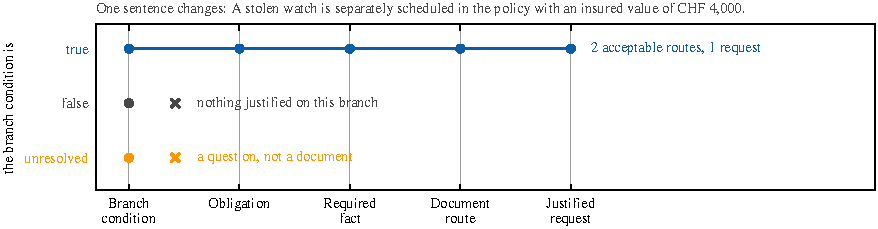
\includegraphics[width=.55\linewidth]{fig_process_principle.pdf}
\caption{\textbf{The active branch controls the request.} A source condition
makes its obligation active, inactive or unresolved. Only an active obligation
reaches a required fact, an evidence capability and a document route;
an unresolved condition yields a clarification question, never the documents
of a branch the case may not be on. New evidence updates the state and the
plan is recomputed. Acquisition permission and route sufficiency are
specified in Section~\ref{sec:method}.}
\label{fig:principle}
\end{figure}

Three questions are usually collapsed into one checklist score, and they
should not be. \emph{Traceability} asks whether a request has an inspectable
chain back to a source. \emph{Branch sensitivity} asks whether changing one
case fact changes exactly the documents that fact justifies.
\emph{Complete-case utility} asks whether a full plan covers what a case needs
without unnecessary demands. None implies the others: a source-linked request
can be wrong, a perfect response to one fact can coexist with errors shared by
both versions of a case, and a plan can look complete while being unjustified.
We evaluate them separately.

Study~A tests branch sensitivity with matched interventions. From a frozen
snapshot of public Swiss insurance law and household-policy wording we build
\nPairsAll{} case pairs whose members differ in one branch-defining statement,
with an independently authored reference contract fixing which signed
document changes are justified. The benchmark is built to fail input-free
shortcuts before any system runs: a constant predictor fitted on the other
branch families scores \pfNoInputMax{} on every held-out family
\citep{gururangan2018artifacts,poliak2018hypothesis,geirhos2020shortcut}.
On the \nPairsHid{} held-out pairs, \casepath makes \cpSpur{} false-positive
signed changes against \dirSpur, \gcSpur{} and \efSpur{} for a direct
predictor, a graph-as-context predictor and an evidence-first pipeline, with
the highest micro-$F_1$ (\cpF), precision (\cpPrec) and exact-pair count
(\cpExactN{} of \nPairsHid). Reassigning its outputs to the wrong branch
families collapses $F_1$ to at most \wpMax. The same frozen report rejects
the preregistered broad-superiority gate: the $F_1$ margins over the two
strongest comparators are below $\gateMargin$ and no family-level test survives Holm
correction. We report both: the method's value is fewer unjustified
requests, not a uniformly better checklist.

Study~B addresses complete-case utility on the entire released corpus:
\nbClaims{} synthetic tenancy claims in \nbFamilies{} families,
\nbLearnedArms{} learned pipelines sharing one compiled public representation
and matched budgets, \nbDependentArms{} dependent controls, and native
endpoints under a frozen finite-corpus contract. Its development phase is
complete and its protected phase is executing at the time of writing
(Section~\ref{sec:native}).

\paragraph{Contributions.}
(1)~An executable evidence semantics: applicability, acquisition permission
and route sufficiency as separate three-valued decisions over a closed
catalogue, so that no document can be requested without a source chain;
evidence ledgers and compiled procedure runtimes already separate semantic
judgement from procedural control \citep{kim2026evidenceobligation,yu2026compile},
and the contribution is the document-planning object and its measured
behaviour.
(2)~A branch-intervention benchmark with built-in falsifiers and a
preregistered gate whose failure we report.
(3)~A matched comparison showing selective, branch-specific and traceable
document changes, with the family-level failures that remain.
(4)~An integrated release: method pack, benchmark, receipts, the
\nbClaims-claim corpus and contract, and a workbench whose replay agrees with
the research planner on all \parityUnits{} benchmark units.

\section{Method: deriving requests from process state}
\label{sec:method}

\subsection{The planning object}
The source specification $K$ records process nodes and their conditions,
obligations, required facts, evidence capabilities and document routes. A
capability describes what the evidence must establish. A route is a subset
of the closed document catalogue $\mathcal D$ that can establish it; a
capability may have several alternative routes. Case state $s=(z,E)$
contains the assessment $z$ of the source conditions and the recorded
evidence $E$. The versioned planner returns documents, a next action and
the chains that justify them:
\begin{equation}
(D_t,a_t,J_t)=\Pi_K(s_t),\qquad s_{t+1}=U(s_t,e_{t+1}),
\label{eq:loop}
\end{equation}
Here $U$ admits an observation or correction and updates the state from
which the next plan is computed. The construction gives two guarantees.
An unresolved condition can produce a question but cannot trigger a
branch-specific document request (non-prematurity). Every document in $D_t$
comes from an active chain containing an obligation, a fact, a capability
and a route (provenance closure).

\subsection{Model judgements and controller decisions}
Model calls perform the semantic work. During preparation, fixed roles
extract propositions anchored to source quotations, synthesise the macro
process, refine propositions into guarded evidence rules and map
capabilities to the document catalogue. At inference time, the interpreter
judges whether each guard holds for the case. These roles return structured
judgements. Code activates obligations, projects requests, selects routes
and prioritises the next action, recording the justification for each
choice (Appendix~\ref{app:studya}). The model can interpret a passage or
assess a condition; document requests must pass through the controller.

\subsection{Study A: guarded rules over a closed catalogue}
\label{sec:v5}
We compiled the frozen Study~A specification from \nPassages{} exact
passages of Swiss insurance law and public household-insurance policies
and forms. The sources are Fedlex, CSS, AXA, Generali, Simpego and the
Swiss Insurance Association; the release records their URLs and content
hashes. Extraction produced \nPropositions{} operational propositions.
A deterministic check requires an evidence rule or an explicit
non-evidentiary classification for each proposition. The resulting
representation contains \nRules{} evidence rules, \nNonEvidentiary{}
non-evidentiary classifications, \nGuards{} case guards and \nCatalogue{}
document types. This completeness check covers the extracted inventory.

Each rule $r$ has a local applicability guard $g_r$, required capabilities
$\mathcal C_r$ and routes $\mathcal R_c$ for each capability $c$. For case
$x$, the interpreter assigns $z_g(x)\in\{\T,\F,\U\}$ to guard $g$.
A true or false verdict requires an exact quotation from that case;
otherwise the verdict becomes unresolved. Missing evidence also leaves a
guard unresolved. Each guard has its own model call, although case packets
are batched for execution, so individual branch decisions remain auditable.
Let $A(x)$ contain the unconditional rules and those whose guards are true.
Let $\mathcal R^{\rm conf}_g$ contain the mapped confirmation routes for a
guard that is true in the narrative but has not been established by admitted
evidence. Given held document types $H$, the planner returns
\begin{equation}
D(x,H)=\Bigl[\bigcup_{r\in A(x)}\bigcup_{c\in\mathcal C_r}\bigcup_{\rho\in\mathcal R_c}\rho
\;\cup\bigcup_{g\ \text{true, unconfirmed}}\ \bigcup_{\rho\in\mathcal R^{\rm conf}_g}\rho\Bigr]\setminus H .
\label{eq:v5}
\end{equation}
Thus a false guard adds no demand, an unresolved guard produces a question,
and the accepted verdicts fully determine the plan. Each request retains
its rule, fact, must-show statement and source spans.

Equation~\ref{eq:v5} also defines this version's limits. V5 unions the
mapped routes: it does not choose one sufficient alternative or assess a
held document's adequacy for a particular capability. Activation depends on
local rule guards. Changing macro-process edges while keeping the rules
and verdicts fixed leaves $D$ unchanged. In Study~A, an ``active path'' is
this case-conditioned applicability structure; it does not require
traversing every graph edge.

\subsection{Study B: applicability, acquisition and adequacy}
\label{sec:native-method}
Study~B deterministically compiles three public tenancy templates into a
representation shared by all arms. It uses no model-based source induction.
The case assessment distinguishes predicate truth, document presence,
individual adequacy and joint adequacy. Activation follows
\begin{equation}
q_s(z)=\phi_s(z)\land_3 J_s\bigl(\{q_p(z)\}_{p\in\mathrm{pa}(s)}\bigr),\ \ 
a_o(z)=q_{\mathrm{scope}(o)}(z)\land_3\phi_o(z),\ \ 
b_o(z)=a_o(z)\land_3\psi_o(z),
\label{eq:native-activation}
\end{equation}
where $J_s$ is the declared all/any join over parent scopes. Roots use the
empty all-join, which is true. The three-valued conjunction $\land_3$ is
false if any input is false, true if all are true and unresolved otherwise.
An obligation's applicability $a_o$ therefore depends on both its enclosing
scope and its own condition. The separate acquisition permission $\psi_o$
must also hold: only $b_o=\T$ permits an immediate request.

A route $\rho$ satisfies capability $c$ only when the required evidence is
present and adequate and the joint assessment is sufficient. Denote this
state by $\rho_c(E)$. Missing or inadequate documents form $M_{c\rho}$;
unknown presence or adequacy creates review items $V_{c\rho}$. The
controller selects
\begin{equation}
\rho_c^*=\operatorname*{arg\,min}^{\rm lex}_{\rho\in\mathcal R_c}
\bigl(\mathbf 1\{\rho_c(E)\ne\T\},\,|M_{c\rho}|,\,|V_{c\rho}|,\,
\operatorname{sort}(M_{c\rho}),\,\operatorname{id}(\rho)\bigr),
\label{eq:native-route}
\end{equation}
independently for each capability, then requests
$\bigcup_c M_{c\rho_c^*}$ over eligible obligations. This is a local route
choice, not a global minimisation. Inactive obligations produce no demand.
Unresolved eligibility produces conditional candidates and questions.
If no route exists, the controller records an evidence gap. Its action
priority is to resolve questions, review evidence, request a document,
review an active gap and, finally, choose an eligible substantive action.

This controller adds sufficiency semantics to the Study~A planning object.
It is a separate runtime, and the experiments do not compare its performance
with V5 or treat it as a repair of V5 (Appendix~\ref{app:correspondence}).

\section{Study A: changing the active branch}
\label{sec:benchmark}

\paragraph{Case pairs and reference changes.}
We selected \nConcepts{} branch concepts for which changing a fact changes
at least one evidence requirement in the sources: a scheduled valuable at
or above the policy threshold, a stolen bicycle, SIM-card theft with misuse,
an identifiable third-party causer, a formal expert procedure, a repair
above the consent threshold, a written demand with a forfeiture period
(\emph{Nachfrist}), recovery of stolen goods and insurer declination.
Each concept appears in four neutral household-theft contexts, giving
\nPairsAll{} pairs and \nUnitsAll{} case units. The two cases in a pair
differ in one statement. For the watch example, ``\pairExampleFalse''
becomes ``\pairExampleTrue''.

Before running any system, we authored a reference contract from the same
sources to specify the acceptable signed changes. It preserves alternatives
such as a receipt or an expert valuation. Both amendments made before the
held-out evaluation remain available with the earlier benchmark versions.
One context per concept supplies \nPairsDev{} development pairs
(\nUnitsDev{} units). The other three contexts, \nPairsHid{} pairs
(\nUnitsHid{} units), stayed sealed until the method, benchmark, analysis
code and gate were hash-frozen, and were read once. This split tests known
rules in new contexts. It does not test transfer to unseen rules or policies.

\paragraph{Controls for shortcut explanations.}
We tested whether static predictions, request volume or branch-independent
changes could explain an apparent gain
\citep{kaushik2018reading,sugawara2018easier,mccoy2019hans,bowman2021benchmarking,yuan2024shortcut}.
A constant signed-set predictor fitted on eight branch families and tested
on the ninth reaches maximum held-out micro-$F_1$ \pfNoInputMax. The nine
target signatures are distinct, with \pfEntropy{} bits of entropy over
\pfUniverse{} signed document atoms.

The wrong-pairing control keeps \casepath's outputs fixed and reassigns them
to other branch families using \wpShifts{} cyclic shifts and \wpDraws{}
seeded derangements. A score that survives this reassignment would not
require branch-specific changes. We also fixed eight acceptance conditions
before the single held-out execution (Table~\ref{tab:gates}), including a
strong requirement for broad superiority.

\paragraph{Scoring.}
For a pair $(x^-,x^+)$, the predicted signed change is
\begin{equation}
\Delta(D)=\{+d:d\in D(x^+)\setminus D(x^-)\}\cup\{-d:d\in D(x^-)\setminus D(x^+)\}.
\label{eq:delta}
\end{equation}
An addition enters with a positive sign and a withdrawal with a negative
sign. The route-aware scorer compares $\Delta$ with each acceptable
reference realisation and selects the best under a frozen lexicographic
rule (Appendix~\ref{app:paired-metrics}). Requesting both alternatives
when one suffices does not receive full credit. We pool true positives,
predictions and reference changes across the \nPairsHid{} pairs to compute
micro precision, recall and $F_1$. A spurious change is an unjustified
addition or withdrawal; a missed change is required but absent. An exact
pair reproduces the entire signed set. These metrics concern changes
between checklists, so a request shared by both cases does not affect them.
We estimate uncertainty with \bootDraws{} bootstrap draws of whole
families and test paired differences with the exact $2^9=\swapAssignments$
family sign-flip test, applying Holm adjustment.

\paragraph{Comparators and computation.}
Direct predicts documents from the case and source material. Graph as
context also receives the induced process and evidence-rule representation,
then generates the document set in one step. Evidence-first derives
evidence needs, retrieves twelve passages by keyword matching and predicts
documents. Every arm uses model setting \texttt{\cpModel}, the same provider
restriction, temperature zero, source snapshot, catalogue and case texts.
The held-out receipts record \dirCalls, \gcCalls, \efCalls{} and \cpCalls{}
calls, respectively. The comparisons hold these inputs and model conditions
fixed, but allow different amounts of computation (Appendix~\ref{app:costs}).

\section{Study A: Selective Branch Adaptation}
\label{sec:paired-results}

\begin{table}[t]
\centering\small
\setlength{\tabcolsep}{5pt}
% GENERATED by evidence/build_manuscript_numbers.py
\begin{tabular}{lrrrrrrr}
\toprule
Method & Prec. & Recall & $F_1$ & Exact & Pred./Gold & Spurious & Missed \\
\midrule
Direct & 0.481 & 0.758 & 0.588 & 0.333 & 52/33 & 27 & 8 \\
Graph as context & 0.431 & 0.939 & 0.590 & 0.148 & 72/33 & 41 & 2 \\
Evidence-first & 0.235 & 0.485 & 0.317 & 0.074 & 68/33 & 52 & 17 \\
\casepath & \textbf{0.615} & 0.727 & \textbf{0.667} & \textbf{0.444} & 39/33 & \textbf{15} & 9 \\
\bottomrule
\end{tabular}

\caption{\textbf{Held-out signed-change evaluation} (\nPairsHid{} pairs,
\nGoldAtoms{} reference changes). Correct, spurious and missed count signed changes. Exact counts pairs
whose entire signed set is reproduced; $F_1$ includes its 95\%
family-cluster bootstrap interval. These are errors in changes between two checklists, not
requests in a complete claim.}
\label{tab:main}
\end{table}



\paragraph{Fewer unjustified changes.}
Table~\ref{tab:main} reports the held-out comparison. \casepath predicts \cpPred{} signed changes for \nGoldAtoms{}
reference changes: \cpTP{} correct, \cpSpur{} spurious, \cpMiss{} missed.
Direct predicts \dirPred{} (\dirTP{} correct, \dirSpur{} spurious), Graph as
context \gcPred{} (\gcTP, \gcSpur) and Evidence-first \efPred{} (\efTP,
\efSpur). \casepath thus makes \redDir\%, \redGc\% and \redEf\% fewer
spurious changes than the three alternatives while keeping recall \cpRec,
and it reproduces the whole signed set on \cpExactN{} of \nPairsHid{} pairs
against \dirExactN, \gcExactN{} and \efExactN. Graph as context recovers the
most reference changes (\gcTP{} of \nGoldAtoms) at the cost of \gcSpur{}
spurious ones. In this comparison, providing the graph as context improves
recall but does not impose the controller's restriction on what may be requested. The contrast with Direct is precise:
twelve fewer false-positive changes for one fewer correct change.

A retrospective partition sharpens the interpretation: \eoCpOutside{} of
\casepath's \cpSpur{} spurious changes concern documents outside the
benchmark's branch-governed set, compared with all \eoDirOutside,
\eoGcOutside{} and \eoEfOutside{} comparator errors. Process control reduces
this form of checklist drift; it does not eliminate it. The partition does
not identify universally required baseline documents, which the signed-change
references do not specify.

\paragraph{How much does the result generalize?}
Family-cluster intervals are wide: $F_1$ \cpF{} $[\cpCIlo,\cpCIhi]$ for
\casepath against $[\dirCIlo,\dirCIhi]$ and $[\gcCIlo,\gcCIhi]$ for the two
strongest comparators, with paired differences $[\dDirLo,\dDirHi]$ and
$[\dGcLo,\dGcHi]$ that include zero; only the contrast with Evidence-first
excludes it ($[\dEfLo,\dEfHi]$). The broad-superiority gate fails on three
of its eight conditions (Table~\ref{tab:gates}): margins \mDir{} and \mGc{}
fall short of $\gateMargin$, precision \cpPrec{} falls short of $\gatePrec$, and the
Holm-adjusted family-swap $p$-values are \pHolmDir, \pHolmGc{} and \pHolmEf.
The count reduction supports selectivity on these pairs; the preregistered
criterion for broad superiority is not met.

\paragraph{Branch specificity.}
Holding \casepath's outputs fixed and pairing them with the wrong branch
families collapses signed-change $F_1$ from \wpObs{} to a maximum of
\wpMax{} over the \wpEvaluated{} evaluated reassignments (mean \wpMean;
add-one randomisation $p=\wpP$). The changes are specific to the intervened
branch. This does not identify the internal representation as the only
possible cause; a family-specific lookup would also pass. Two structural
facts are separate from accuracy: all \chainAttributed{} of \chainPredicted{}
predicted changes are attributed in the retained records to a changed guard,
including the incorrect ones, and \chainCovered{} of \nGoldAtoms{} reference
changes (\chainCoverage\%) are reachable through a source chain in the frozen
representation. Attribution is an invariant of the architecture, not evidence
that a mapping was right; reachability says a route existed, not that it was
emitted.

\begin{figure}[t]
\centering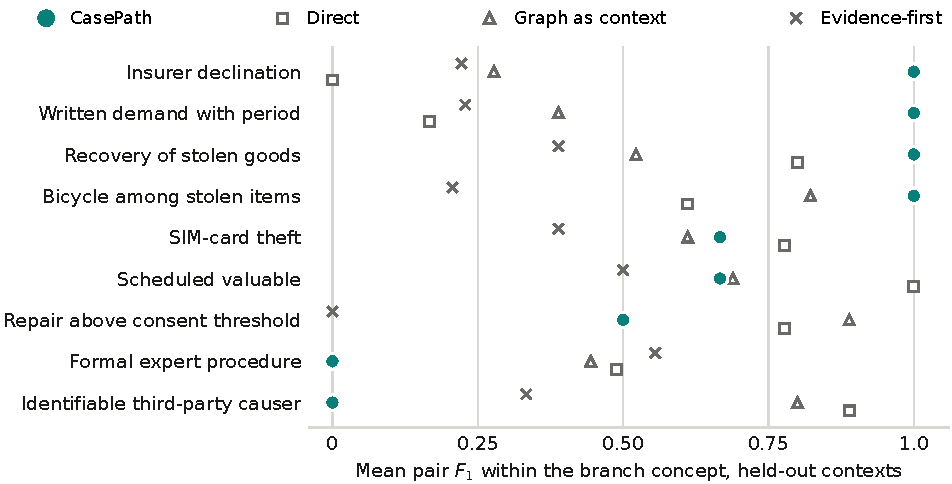
\includegraphics[width=\linewidth]{fig_family_results.pdf}
\caption{\textbf{Where the semantics holds and where it fails.} Mean pair
$F_1$ per branch concept on the held-out contexts: the marker is \casepath,
the square, triangle and cross identify Direct, Graph as context and
Evidence-first. Small vertical offsets separate coincident values. \casepath is
exact on \nFamExact{} concepts where the comparators are not, and scores zero
on \nFamZero{} where they succeed. Concepts are ordered by \casepath's score,
so the failures sit at the bottom beside the comparators that solved them.}
\label{fig:family}
\end{figure}

\paragraph{Procedural branches explain the advantage.}
Figure~\ref{fig:family} shows the structure the aggregate hides. \casepath is
exact on all three held-out contexts of \nFamExact{} concepts (bicycle, declination,
recovery, \emph{Nachfrist}), reaches $\cpFamScheduled$ on scheduled valuables and
SIM-card theft, $\cpFamRepair$ on repair consent, and scores zero on third-party
causation and the formal expert procedure. The zeros are systematic rather
than random: an alternative route is over-requested where one would suffice,
a condition is attached at the wrong semantic granularity, or an adjacent
procedural guard activates the wrong confirmation document. The
comparators are strong where the plausible claimant document is the right
answer (third party, repair consent) and weak where the justified change is a
procedural artefact that a checklist prior does not suggest (declination,
\emph{Nachfrist}); per-concept values are in Appendix~\ref{app:family}.
Finally, a change metric is blind to a document omitted or over-requested in
both members of a pair, and these cases are rule units rather than whole
claims; Study~B therefore scores complete plans on whole cases.

\FloatBarrier
\section{Study B: Complete Claims and the Value of Process Scope}
\label{sec:native}

\paragraph{A matched complete-corpus comparison.}
Study~B evaluates all \nbClaims{} released synthetic tenancy claims across
\nbFamilies{} families in three domains: defects, mould and heating;
termination; and rent increase. Development contains \nbDevClaims{} claims
in \nbDevFamilies{} families; the protected split contains \nbHidClaims{}
claims in \nbHidFamilies{} disjoint families. Five learned pipelines share
the compiled public representation, observable packet, source access,
model alias and budget: \nbCallsPerCell{} calls per cell, \nbReasoning{}
reasoning, \nbTokens{} completion tokens per call, no tools or resampling.
\casepath emits an assessment that code compiles into the artefact;
Direct, Document-first, Process-context and Rule-first generate the artefact.
Compiled-equivalent and local-scope controls reuse \casepath's assessments.
This compares complete pipelines under matched information and budget.

\paragraph{Registered primary and separately specified analyses.}
All \nrArtifactFailures{} generated artefacts fail the original native
interface: the compiler's condition names are not bound in the reference
scenario. The frozen policy penalizes all \nbCells{} cells, including
\nrRequestPenalties{} failed or blocked outputs; \nrPrimaryMet{} of
\nrPrimaryTotal{} protected-split practical targets are met. The primary
report and failures remain unchanged. Two retrospective analyses answer
narrower questions: whether literal requests agree with reference sets, and
whether inherited scope improves a plan evaluated at its recorded assessed
state. Neither replaces the registered result.

\paragraph{Realized request quality across all pipelines.}
The first analysis scores literal immediate requests with the original
reference and counting functions, without interpreting guards. All
\nrRequestObserved{} generated lists are scoreable; failed outputs retain
zero quality scores and an unnecessary-fraction penalty of one.
Table~\ref{tab:native-final} shows the complete comparison. \casepath produces
\rqHidCpN{} lists on protected families, with failure-penalized $F_1$
\rqHidCpF{} against \rqHidPcF{} for the strongest comparator,
Process-context. The difference includes output availability: the
conventional paired advantage is \rqHidDPcF, but the conservative contrast,
assigning $-1$ whenever either endpoint is unobserved, is \rqHidCPcF.
This supports better realized output under the budget, not reliable paired
superiority over the learned alternatives.

\begin{table}[t]
\centering\small
\setlength{\tabcolsep}{4pt}
\begin{tabular}{lrrrrrr}
\toprule
& \multicolumn{2}{c}{Generated lists} & \multicolumn{2}{c}{Checklist $F_1\uparrow$} & \multicolumn{2}{c}{Unnecessary$\downarrow$} \\
\cmidrule(lr){2-3}\cmidrule(lr){4-5}\cmidrule(lr){6-7}
Pipeline & Dev. & Prot. & Dev. & Prot. & Dev. & Prot. \\
\midrule
\casepath & \rqDevCpN & \rqHidCpN & \rqDevCpF & \rqHidCpF & \rqDevCpU & \rqHidCpU \\
Direct & \rqDevDirN & \rqHidDirN & \rqDevDirF & \rqHidDirF & \rqDevDirU & \rqHidDirU \\
Document-first & \rqDevDocN & \rqHidDocN & \rqDevDocF & \rqHidDocF & \rqDevDocU & \rqHidDocU \\
Process-context & \rqDevPcN & \rqHidPcN & \rqDevPcF & \rqHidPcF & \rqDevPcU & \rqHidPcU \\
Rule-first & \rqDevRfN & \rqHidRfN & \rqDevRfF & \rqHidRfF & \rqDevRfU & \rqHidRfU \\
\midrule
\multicolumn{7}{l}{\textit{Dependent controls: same recorded CasePath assessments}} \\
Compiled equivalent & \rqDevCeN & \rqHidCeN & \rqDevCeF & \rqHidCeF & \rqDevCeU & \rqHidCeU \\
Local-scope ablation & \rqDevLsN & \rqHidLsN & \rqDevLsF & \rqHidLsF & \rqDevLsU & \rqHidLsU \\
\bottomrule
\end{tabular}

\caption{\textbf{Complete-corpus request comparison.} Retrospective agreement
of literal request lists with reference sets. Scores weight domains equally,
families equally within domains and cases equally within families. Failed
outputs remain in the denominator; ``Unnecessary'' includes their unit
penalty. Dependent controls reuse the same recorded assessments.}
\label{tab:native-final}
\end{table}

\paragraph{Making the assessed state explicit.}
The second analysis specializes each saved artefact to its own authenticated
assessment. A condition known true activates its entities; a false condition
does not; unresolved entities remain recorded as unresolved and are not
asserted active. The resulting current-case snapshot can be scored without
substituting the reference scenario for the model's beliefs. The original
requests and all failed cells are retained. Only \casepath and its two
dependent controls have the required saved assessments. Every available
snapshot scores successfully, and none excludes a literal immediate request.
This interface evaluates current-case structure, not the program's response
to hypothetical branch changes (Appendix~\ref{app:assessed-state}).

\begin{figure}[t]
\centering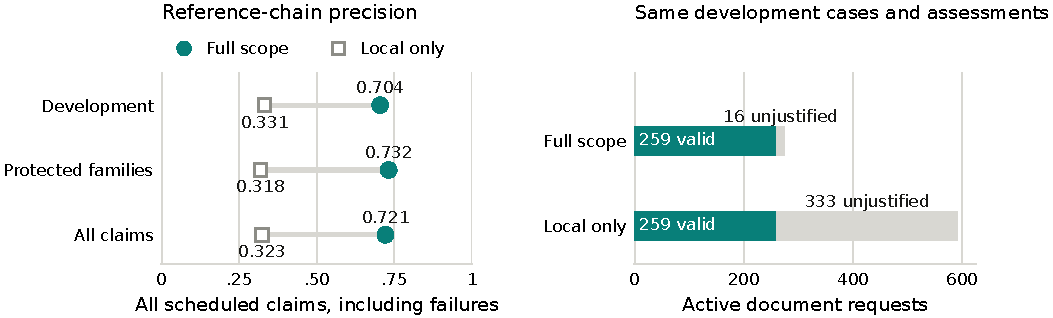
\includegraphics[width=\linewidth]{fig_scope_control.pdf}
\caption{\textbf{Inherited scope removes unjustified demand.} Left:
reference-chain precision in the retrospective current-case evaluation,
including every scheduled case and failure penalty. Right: on the same
\asDevCpN{} completed development cases, both controllers retain
\asDevCpValid{} valid requests; enclosing scope reduces total requests
from \asDevLsReq{} to \asDevCpReq. The assessment and source representation
are fixed.}
\label{fig:scope}
\end{figure}

\paragraph{The benefit is selectivity at fixed assessment.}
Figure~\ref{fig:scope} isolates inherited domain scope: an obligation must
satisfy the enclosing process conditions as well as its local guard.
On protected families, native valid-chain precision rises from
\asHidLsChain{} to \asHidCpChain; the conservative paired benefit remains
positive at \asHidCChain{} even after penalizing unavailable pairs. The
corresponding unnecessary fraction falls from \asHidLsU{} to
\asHidCpU. These are complementary views of the same requests, not
independent effects. On the same \asDevCpN{} completed development cases,
both controllers recover \asDevCpValid{} valid requests, while total
requests fall from \asDevLsReq{} to \asDevCpReq. Scope therefore removes
unjustified demands without sacrificing those recovered obligations.
The compiled-equivalent control matches \casepath exactly. The intervention
establishes the value of inherited domain applicability; it does not isolate
arbitrary graph topology. Native chain matching checks agreement with
reference decision--fact--capability--document links, not exact-source
entailment: provenance-chain inheritance is zero in both controllers.

The family label records the original target-custody split: observable
inputs had been inspected during product work, historical target non-access
is not established because the producer's complete I/O audit is missing,
and targets are now released. These are finite-corpus descriptive analyses,
not fresh hidden confirmation. Costs are \$\nrStudyCost{} for the study and
\$\nrTotalCost{} including earlier activity; the retrospective analyses add
no provider calls. Full endpoints, raw counts and paired contrasts are in
Appendix~\ref{app:request-diagnostic} and Appendix~\ref{app:assessed-state}.

\FloatBarrier
\section{Related Work}
\label{sec:related}

\paragraph{Executable rules and adaptive case state.}
LegalRuleML represents norms with their source associations
\citep{oasis2021legalruleml}; Catala makes legislative computation
executable \citep{merigoux2021catala}; DMN formalises decisions and CMMN
guard-activated case work \citep{omg2024dmn,omg2016cmmn}; Guard--Stage--Milestone
models and DCR reference models of law connect data-driven activation to
compliance \citep{vaculin2011gsm,lopez2020dcrlaw}; proactive enforcement
derives actions from active obligations \citep{basin2024proactive}; and
insurance software conditions document lists on service definitions
\citep{servicenow2026documentlists}. These are prior art; \casepath adds
their explicit coupling to language-model assessments and a measurement of
the resulting evidence-planning errors.

\paragraph{Procedure extraction and process-guided agents.}
PAGED extracts procedural graphs from documents \citep{du2024paged}; BREX
benchmarks business-rule flows with executable grounding \citep{yang2026brex};
Guideline2Graph compiles clinical guidelines into provenance-preserving
decision graphs \citep{kilic2026guideline2graph}; \citet{graus2026decisionmodels}
evaluate structured representations for legal decision models; CANONIC frames
governance as compilation \citep{hadley2026canonic}. FlowBench and WorFBench
evaluate workflow-guided planning and workflow generation
\citep{xiao2024flowbench,qiao2024worfbench}; Procedural Graphs localise an
agent to an active node \citep{lu2026proceduralgraphs}; ReAct interleaves
reasoning and action \citep{yao2022react}. None scores whether a changed
case fact changes exactly the justified evidence.

\paragraph{Obligation-controlled acquisition.}
The closest precedents are \citet{kim2026evidenceobligation}, whose evidence
ledger activates branch-specific knowledge obligations while a model judges
semantic warrant and code manages closure, and \citet{yu2026compile}, who
compile SOP constraints into verification routines with evidence-bearing
returns and an active execution frame. \casepath's residual is the
document-planning object: applicability separated from acquisition
permission, presence from capability-specific and joint adequacy,
alternative routes kept as alternatives, and a benchmark that tests the
consequence downstream. Neither system is reproduced as an arm, and no
superiority over them is claimed.

\paragraph{Grounding, evidence and information seeking.}
GraphCompliance aligns policy and context graphs for regulatory assessment
\citep{chung2025graphcompliance}; CLER scores litigation evidence lists and
the facts they prove \citep{bi2026cler}; InfoGatherer selects retrieval and
questions by evidential uncertainty \citep{taranukhin2026infogatherer};
verified quotation and chain-of-verification make support inspectable
\citep{menick2022verifiedquotes,dhuliawala2024chain}. Tool-use benchmarks
score whether the right function was called \citep{li2023apibank,patil2025bfcl},
the analogue of asking for a plausible document; \casepath asks whether the
call was justified by the case.

\paragraph{Benchmark validity.}
Partial-input baselines, annotation artefacts and shortcut learning motivate
the input-free control and the wrong-pairing permutation
\citep{kaushik2018reading,poliak2018hypothesis,gururangan2018artifacts,mccoy2019hans,sugawara2018easier,geirhos2020shortcut,bowman2021benchmarking,yuan2024shortcut}.
Study~A's references are authored from sources rather than adjudicated by a
model, avoiding the preference leakage that arises when judged and judging
models coincide \citep{li2026preference}; work on evaluation validity
\citep{thomas2026validity} and critiques of legal benchmarks that reward
outcome prediction over practitioners' work
\citep{medvedeva2023right,lou2026lawyering} motivate signed document changes
and emitted requests as the measured objects.

\section{Research and product correspondence}
\label{sec:release}

The Study~A product uses the experiment's guard interpreter and planner.
Its hash-bound method pack contains the frozen representation,
propositions, source snapshot, method manifest, benchmark identity and
model configuration. Clients cannot supply rules, mappings or targets;
the endpoint rejects hash drift. The interface exposes the guard states
and justification chains alongside questions, gaps, requests, exact source
spans and the next action.

To check this correspondence, we replayed all \parityUnits{} benchmark
units through the product with their recorded guard decisions. Every
unit reproduced the research document set, guard states and next action,
as did all \parityPairs{} signed pair changes. Every displayed quotation
was an exact substring of its source passage. This verifies implementation
identity conditional on the recorded assessments; fresh model agreement
and hosted deployment identity require separate checks.

The workbench organises Facts, Orchestration, Source Integrity, Process,
Evidence, and Audit and Readiness around one case record. Admitting a new
observation recomputes the plan through Equation~\ref{eq:loop}. The release
contains the benchmark versions, predictions, receipts, analysis code and
parity verifier, together with Study~B's corpus, producer, evaluator,
contract and every recorded cell. The registered primary failure and the
separate request-only diagnostic reproduce offline from the exact released
reference containers. Reference targets, authored teaching states and model
predictions appear separately; the first two supply no additional benchmark
evidence.

\section{Discussion and Limitations}
\label{sec:limitations}

The practical value of process control is selectivity with an inspectable
reason. In Study~A, \casepath removes false-positive changes while retaining
nearly as many correct changes as Direct. The benefit is largest on
procedural branches, where a familiar claimant document is a poor substitute
for the particular notice or confirmation that the rule requires. Study~B's
current-case scope intervention establishes a related design choice: an obligation
must inherit the conditions of its enclosing process, not merely satisfy its
own local condition. A system builder can inspect and test both dependencies
before asking a customer for another document.

The evidence has specific limits. Study~A tests known concepts in new
contexts and additions rather than justified withdrawals, uses unequal computation across pipelines, and does not meet its
preregistered broad-superiority gate. Its source-derived references contain
author judgements about which documents establish a fact, rather than expert
consensus; a deployed system would also need to select the governing policy
instead of combining rules from multiple insurers. Study~B tests complete
synthetic claims under matched budgets, but its native interface failure
leaves counterfactual graph correctness unvalidated. Its retrospective
current-case analysis isolates scope within dependent controls; the broader
request comparison measures realized output under failures.
Neither study measures customer effort, expert agreement, autonomous
acquisition or performance in another jurisdiction.

\section{Conclusion}
\label{sec:conclusion}

Evidence planning benefits from making the reason for a request executable.
\casepath represents the dependency from source condition to obligation,
fact, capability and document, and lets case state determine which demands
are active. The controlled comparison finds fewer unjustified checklist
changes; the current-case intervention shows that inherited scope removes
unjustified demand while retaining the same recovered obligations in development. These results support a concrete design
principle: derive evidence demands from explicit, case-conditioned
obligations, and validate both the requests and the process semantics that
produce them. The released benchmarks, controller, traces and offline
reproduction make that principle inspectable and testable.

\label{end-of-main-text}
\section*{Reproducibility statement}
For Study~A, the release includes the frozen source snapshot, propositions,
rules, document map, interpreter and planner, along with every benchmark
version, prediction, provider receipt, analysis script, preregistered gate
and product replay verifier. For Study~B, it includes the corpus, compiled
representation, producer, evaluator, analysis contract and every recorded
cell, including failures. Scripts generate each numerical result in the
paper and record its source-file hash and JSON pointer. The release
commands recompute Study~A and all three Study~B analyses from the saved
outputs, comparing them with the preserved measurements without network or
provider access (Appendices~\ref{app:studya} and~\ref{app:request-diagnostic}).
Regenerating the model outputs would require provider access and would not
be deterministic.

\section*{Ethics statement}
The studies use public-source snapshots and synthetic cases containing no
personal data. \casepath is a research architecture for evidence planning;
it provides neither legal advice nor automated coverage decisions. Use in
practice would require policy and jurisdiction scoping, professional review,
privacy controls, and procedures for correction and appeal.

\section*{AI use statement}
We used generative AI in hypothesis formulation, methodological critique,
literature discovery, implementation and testing, synthetic-case construction,
diagnostic interpretation, and the drafting and editing of text and figures.
The reproducibility materials identify actual executions, engineering
fixtures, archived reports and author judgements, and retain failed results
and version differences. The authors take responsibility for the final
claims, citations, measurements and artefacts.

\bibliography{references}
\bibliographystyle{iclr2027_conference}
\appendix
\section{Study A: Benchmark and Analysis Details}
\label{app:studya}

\paragraph{Branch concepts.}
The \nConcepts{} concepts are: a scheduled valuable at or above the
source-defined threshold; a bicycle or e-bike among the stolen items;
SIM-card theft with a misuse claim; an identifiable third-party causer;
selection of formal expert proceedings; contemplated repairs above the
consent threshold; a written demand with a forfeiture warning and period;
recovery of, or news about, stolen items; and insurer declination. Each has
four neutral contexts; a pair changes only the branch statement.

\paragraph{Signed-change scoring.}
\label{app:paired-metrics}
For pair $i$ the scorer evaluates each acceptable signed reference
realisation $G\in\mathcal G_i$ against the prediction $P_i=\Delta(D_i)$ and
selects the maximum of the lexicographic tuple
$\bigl(F_1(P_i,G),\,|P_i\cap G|,\,\mathrm{Prec}(P_i,G),\,\mathrm{Rec}(P_i,G),\,-|G|,\,\mathrm{sort}(G)\bigr)$,
whose last component is the frozen deterministic tie-break. Precision and
recall use zero for empty denominators; $F_1$ is one when prediction and
reference are both empty. Micro scores pool the selected realisation counts
across the \nPairsHid{} pairs; family means average pair $F_1$ within each
of the nine concepts. The family bootstrap resamples nine whole families
with replacement on each of \bootDraws{} draws (seed \bootSeed), retaining
all three held-out contexts of each selected family. The exact family-swap
test enumerates \swapAssignments{} sign assignments of the nine family mean
differences; the three one-sided $p$-values (\pRawDir, \pRawGc, \pRawEf)
receive Holm adjustment (\pHolmDir, \pHolmGc, \pHolmEf). The wrong-pairing
diagnostic uses \wpShifts{} cyclic shifts and \wpDraws{} sampled
derangements with add-one score $(1+N_{\ge})/(1+\wpEvaluated)$; the reported
maximum is over this evaluated collection, not all derangements.

\paragraph{Per-concept results.}
\label{app:family}
Table~\ref{tab:family} lists the held-out mean pair $F_1$ for every branch
concept and arm.
\begin{table}[htb]
\centering\small
% GENERATED by evidence/build_manuscript_numbers.py
\begin{tabular}{lcccc}
\toprule
Branch concept & Direct & Graph ctx. & Evid.-first & \casepath \\
\midrule
Bicycle among stolen items & 0.611 & 0.822 & 0.206 & 1.000 \\
Insurer declination & 0.000 & 0.278 & 0.222 & 1.000 \\
Formal expert procedure & 0.489 & 0.444 & 0.556 & 0.000 \\
Recovery of stolen goods & 0.800 & 0.522 & 0.389 & 1.000 \\
Written demand with period (Nachfrist) & 0.167 & 0.389 & 0.229 & 1.000 \\
Repair above consent threshold & 0.778 & 0.889 & 0.000 & 0.500 \\
Scheduled valuable & 1.000 & 0.689 & 0.500 & 0.667 \\
SIM-card theft & 0.778 & 0.611 & 0.389 & 0.667 \\
Identifiable third-party causer & 0.889 & 0.800 & 0.333 & 0.000 \\
\bottomrule
\end{tabular}

\caption{Held-out mean pair $F_1$ by branch concept.}
\label{tab:family}
\end{table}

\paragraph{Preregistered gate.}
Table~\ref{tab:gates} lists the eight conditions fixed before the one-shot
read and their outcomes.
\begin{table}[htb]
\centering\small
% GENERATED by evidence/build_manuscript_numbers.py
\begin{tabular}{p{0.80\linewidth}c}
\toprule
Preregistered held-out gate & Result \\
\midrule
$F_1$ margin $\geq 0.10$ against every comparator & fail \\
Holm-adjusted family-swap $p\leq 0.05$ against every comparator & fail \\
Signed-change precision $\geq 0.70$ & fail \\
Predicted/gold change ratio in $[0.75,1.50]$ & pass \\
Predicted changes attributed to a changed guard $\geq 0.90$ & pass \\
Reference changes reachable through a source chain $\geq 0.80$ & pass \\
Correct pairing above the wrong-pairing 97.5th percentile & pass \\
No requested document without a source chain & pass \\
\bottomrule
\end{tabular}

\caption{Preregistered held-out gate, fixed before the one-shot read. The
provenance, volume and pairing conditions pass; the broad-superiority
conditions do not.}
\label{tab:gates}
\end{table}

\paragraph{Frozen record and development separation.}
The method freeze \path{casepath.theft-method-freeze/5.0.0} binds source
bytes, benchmark v3 and both amendments, the proposition-complete refinement,
document mapping, interpreter V4, planner V3, model, provider and temperature
settings, analysis code, the development split, the matched comparators' raw
predictions and the focused method tests. Development used \nPairsDev{}
pairs (\nUnitsDev{} units), one context per concept, and its predeclared
admission checks authorised exactly one held-out read of the remaining
\nPairsHid{} pairs (\nUnitsHid{} units) under a separately hash-bound
execution freeze. After the held-out result, the method was marked locked
and no scientific file was adapted from held-out outcomes.

\paragraph{Calls and recorded costs.}
\label{app:costs}
Table~\ref{tab:costs} lists the held-out provider receipts per arm.
\begin{table}[htb]
\centering\small
% GENERATED by evidence/build_manuscript_numbers.py
\begin{tabular}{lrrrrr}
\toprule
Arm & Calls & Prompt tokens & Completion tokens & Max completion & Cost (USD) \\
\midrule
Direct & 54 & 2,900,625 & 45,678 & 14,000 & 4.83 \\
Graph as context & 54 & 5,345,421 & 42,663 & 14,000 & 8.41 \\
Evidence-first & 108 & 259,890 & 66,450 & 14,000/18,000 & 1.06 \\
\casepath & 87 & 1,005,211 & 243,891 & 10,000 & 5.44 \\
\bottomrule
\end{tabular}

\caption{Held-out provider receipts, one logged attempt per call, model
\texttt{\cpModel}, temperature $0$. Evidence-first allows \efMaxTokExtract{} completion
tokens for extraction and \efMaxTokPlan{} for planning; \casepath allows \cpMaxTokGuard{} per
guard batch; Direct and Graph as context allow \dirMaxTokCall{} per call. Costs are provider-reported charges, exclusive of source
preparation; the arms are not compute-matched.}
\label{tab:costs}
\end{table}

\paragraph{Product-parity contract.}
The parity verifier loads the installed hash-bound method pack and the real
product service, replays all \parityUnits{} units with the recorded guard
decisions, compares guard verdicts, document sets and next actions, compares
all \parityPairs{} pair deltas through the product diff surface, and checks
that every rendered quotation is an exact substring of its source passage.
A successful HTTP response or a plausible demo is not treated as evidence of
implementation identity.

\section{Versioned Correspondence Between the Two Studies}
\label{app:correspondence}
\begin{table*}[t]
\centering\small
\setlength{\tabcolsep}{4pt}
\renewcommand{\arraystretch}{1.09}
\begin{tabularx}{\textwidth}{@{}>{\raggedright\arraybackslash}p{.17\textwidth}>{\raggedright\arraybackslash}X>{\raggedright\arraybackslash}X@{}}
\toprule
Binding & Study A: theft-method-freeze/5.0.0 & Study B: native-150 compact controller \\
\midrule
Knowledge & Source-extracted propositions, macro graph, refined local evidence rules and mapped routes & Common deterministic compilation of all three public tenancy templates \\
Online gate & Rule-local true/false/unresolved guard; macro edges do not gate requests & Inherited applicability scopes, obligation condition and separate acquisition permission \\
Evidence state & Held document types; true-guard confirmation; union of mapped routes & Presence, capability/route adequacy, multi-document joint adequacy; per-capability route selection \\
State update & Recompute requests/next action from a changed packet; paired edit, not acquired evidence outcome & Recompute from a new assessment; benchmark measures one planning realization \\
Population & 9 development + 27 held-out pairs; nine shared concepts, four contexts; 72 units total & 60 development/11 families + 90 protected/17 families; 150 claims, three tenancy domains \\
Learned inference & Guard-major batched V5; 1-call Direct, 1-call representation baseline, 2-call Evidence-first & Five 2-call singleton pipelines; two additional controls reuse CasePath state \\
Endpoint & Route-aware signed additions/withdrawals, 27-pair micro scores & Complete native artifact and separate actual immediate-checklist metrics \\
Analysis & Historical family bootstrap, exact family swaps and wrong-family diagnostic; broad gate failed & Equal domain/family/case finite contrasts; family-deletion sensitivity, no significance claim \\
Parity & Recorded-answer replay over 72 units and 36 deltas & Separate implementation; no inherited V5 or six-role/live-app parity claim \\
\bottomrule
\end{tabularx}
\caption{A common source-to-state-to-evidence interface does not make the two
implementations, populations or measurements interchangeable. Study B extends
the evidence question rather than retrospectively re-evaluating V5.}
\label{tab:full-correspondence}
\end{table*}


The shared interface is source specification, case assessment, evidence
planning, state replacement and a justified next action. It does not assert
identical knowledge, algorithms, estimands or validation across the two
implementations. Study~A is bound to
\path{casepath.theft-method-freeze/5.0.0}, interpreter V4 and evidence
overlay V3; Study~B is bound to the compact native producer and its
\texttt{obligation\_control\_v1} and \texttt{evidence\_demand\_v1}
controller. The native public template union is not a transfer of the theft
source pack, and the theft pairs are not transformations of the native claim
roster. V5 judges local guards and projects every mapped route on active
rules plus mapped confirmation evidence for true unconfirmed guards, minus
held document types; it implements neither capability-specific nor joint
adequacy. The native controller distinguishes applicability from
acquisition, unknown from missing evidence, and per-capability route
selection from route union. These are substantive version differences, and
no benchmark comparison between the runtimes is claimed. Study~A's
preparation extracted propositions, synthesised and refined rules and mapped
capabilities with model calls and retained source-only corrections; its
reported held-out costs exclude that preparation. Study~B's compilation is
deterministic and shared by all arms.

\section{Study B: Native Measurements and Analysis Contract}
\label{app:native-metrics}

\paragraph{Native endpoints.}
Native critical-evidence recall is criticality-weighted coverage of active
evidence obligations through any complete permitted document alternative.
Evidence-obligation completeness additionally requires valid
decision--fact--capability--document relations. Valid-chain precision counts
requested items with such a chain over all requested items; its empty-set
value is one and must be read beside coverage. Wrong-branch and premature
requests, document states, node and edge scores, branch and path probes and
source locators retain their native contracts; locator agreement is not
semantic entailment, and probe accuracy is not a direct measure of inferred
case-predicate accuracy. The emitted endpoint counts unique immediate
request identities without activating candidate conditions from the
reference scenario, and is available only when the reference has a unique
allowed document set for every active obligation, complete consistent
document states and the public label mapping. For predicted and reference
sets $P,G$: $F_1=2|P\cap G|/(|P|+|G|)$ and unnecessary fraction
$U=|P\setminus G|/|P|$; both-empty $F_1$, empty-prediction precision and
empty-reference recall are one, and empty-prediction burden is zero. Failed
cells use adverse frozen unit penalties instead: zero for higher-is-better
rates, one for lower-is-better rates. Unavailable reference labels never
become empty sets or silently shrink a denominator.

\paragraph{Estimation.}
For a split or the complete corpus, each scheduled case has weight
$\omega_i=1/(3\,m_{d(i)}\,n_{f(i)})$, where $m_d$ is its domain's family
count and $n_f$ its family's scheduled case count. Conventional differences
use adverse-imputed unit scores; conservative benefit-oriented differences
contribute $-1$ whenever either producer endpoint is unobserved. Every
single-family deletion is reported with remaining weights renormalised
within the affected domain; these ranges are composition sensitivity, not
confidence intervals. A comparator is counted as beaten only when all three
conservative contrasts strictly exceed their boundaries on the complete
protected population under the original references and integrity checks;
otherwise the report labels the outcome as not met, a partial practical
signal, or not evaluable.

\paragraph{Execution and failure classes.}
Each cell records its arm, case, state and either the validated artefact or
the retained provider output with the reason validation failed. Unknown
relation endpoint: a candidate artefact relation references a node identity
that does not exist in the artefact. Truncated or non-terminal: the
completion reached the \nbTokens-token limit or ended without a terminal
outcome. Invalid codebook index: a reference into the shared public codebook
that does not resolve. Contradictory presence state: a document marked both
present and absent, or present with an inconsistent state. Blocked
dependency: a dependent control whose \casepath source cell failed. Every
failure retains its charge; a repaired version can never replace a failed
cell in the frozen comparison.

\section{Post-hoc Request-Only Diagnostic}
\label{app:request-diagnostic}

The registered wrapper scores emitted requests only after a native receipt
has no evaluation failures. A common expression-namespace mismatch therefore
suppresses request scoring for every generated artefact. The post-hoc
diagnostic changes that availability rule alone: it reads the unchanged
\texttt{request\_mode=now} items, maps their labels with the original public
mapping, and applies the original emitted-set scorer. It never evaluates a
candidate condition against a reference state. All original artefacts,
producer failures, native failures, primary penalties and costs remain
separately available.

All \nbClaims{} references yield an eligible unique document set. The
\nrRequestObserved{} generated lists receive observed request-only scores;
\nrRequestPenalties{} failed or blocked outputs receive the original adverse
checklist penalties, with no invented requests. Domain--family--case
weighting is unchanged. For benefit direction $b_m\in\{-1,1\}$, the
conventional paired contribution is
$b_m(s_{i,\mathrm{CP},m}-s_{i,a,m})$; the conservative contribution is the
same quantity when both request-only endpoints are observed and $-1$
otherwise. A graph's native failure does not make an independently scoreable
request list unobserved in this diagnostic. No practical threshold,
significance test or confidence interval is applied.

\begin{table}[htb]
\centering\small
\setlength{\tabcolsep}{4pt}
\begin{tabular}{lrrrrrr}
\toprule
\multicolumn{7}{l}{\textbf{Development: 60 claims}} \\
Pipeline & Lists & Correct/req. & Missed & Cond. & Prec. & Recall \\
\midrule
\casepath & \rqDevCpN & \rqDevCpCorrect/\rqDevCpRequested & \rqDevCpMissed & \rqDevCpConditional & \rqDevCpP & \rqDevCpR \\
Direct & \rqDevDirN & \rqDevDirCorrect/\rqDevDirRequested & \rqDevDirMissed & \rqDevDirConditional & \rqDevDirP & \rqDevDirR \\
Document-first & \rqDevDocN & \rqDevDocCorrect/\rqDevDocRequested & \rqDevDocMissed & \rqDevDocConditional & \rqDevDocP & \rqDevDocR \\
Process-context & \rqDevPcN & \rqDevPcCorrect/\rqDevPcRequested & \rqDevPcMissed & \rqDevPcConditional & \rqDevPcP & \rqDevPcR \\
Rule-first & \rqDevRfN & \rqDevRfCorrect/\rqDevRfRequested & \rqDevRfMissed & \rqDevRfConditional & \rqDevRfP & \rqDevRfR \\
Compiled equivalent & \rqDevCeN & \rqDevCeCorrect/\rqDevCeRequested & \rqDevCeMissed & \rqDevCeConditional & \rqDevCeP & \rqDevCeR \\
Local-scope ablation & \rqDevLsN & \rqDevLsCorrect/\rqDevLsRequested & \rqDevLsMissed & \rqDevLsConditional & \rqDevLsP & \rqDevLsR \\
\bottomrule
\end{tabular}
\par\medskip
\begin{tabular}{lrrrrrr}
\toprule
\multicolumn{7}{l}{\textbf{Protected families: 90 claims}} \\
Pipeline & Lists & Correct/req. & Missed & Cond. & Prec. & Recall \\
\midrule
\casepath & \rqHidCpN & \rqHidCpCorrect/\rqHidCpRequested & \rqHidCpMissed & \rqHidCpConditional & \rqHidCpP & \rqHidCpR \\
Direct & \rqHidDirN & \rqHidDirCorrect/\rqHidDirRequested & \rqHidDirMissed & \rqHidDirConditional & \rqHidDirP & \rqHidDirR \\
Document-first & \rqHidDocN & \rqHidDocCorrect/\rqHidDocRequested & \rqHidDocMissed & \rqHidDocConditional & \rqHidDocP & \rqHidDocR \\
Process-context & \rqHidPcN & \rqHidPcCorrect/\rqHidPcRequested & \rqHidPcMissed & \rqHidPcConditional & \rqHidPcP & \rqHidPcR \\
Rule-first & \rqHidRfN & \rqHidRfCorrect/\rqHidRfRequested & \rqHidRfMissed & \rqHidRfConditional & \rqHidRfP & \rqHidRfR \\
Compiled equivalent & \rqHidCeN & \rqHidCeCorrect/\rqHidCeRequested & \rqHidCeMissed & \rqHidCeConditional & \rqHidCeP & \rqHidCeR \\
Local-scope ablation & \rqHidLsN & \rqHidLsCorrect/\rqHidLsRequested & \rqHidLsMissed & \rqHidLsConditional & \rqHidLsP & \rqHidLsR \\
\bottomrule
\end{tabular}
\par\medskip
\begin{tabular}{lrrrrrr}
\toprule
\multicolumn{7}{l}{\textbf{Combined: 150 claims}} \\
Pipeline & Lists & Correct/req. & Missed & Cond. & Prec. & Recall \\
\midrule
\casepath & \rqAllCpN & \rqAllCpCorrect/\rqAllCpRequested & \rqAllCpMissed & \rqAllCpConditional & \rqAllCpP & \rqAllCpR \\
Direct & \rqAllDirN & \rqAllDirCorrect/\rqAllDirRequested & \rqAllDirMissed & \rqAllDirConditional & \rqAllDirP & \rqAllDirR \\
Document-first & \rqAllDocN & \rqAllDocCorrect/\rqAllDocRequested & \rqAllDocMissed & \rqAllDocConditional & \rqAllDocP & \rqAllDocR \\
Process-context & \rqAllPcN & \rqAllPcCorrect/\rqAllPcRequested & \rqAllPcMissed & \rqAllPcConditional & \rqAllPcP & \rqAllPcR \\
Rule-first & \rqAllRfN & \rqAllRfCorrect/\rqAllRfRequested & \rqAllRfMissed & \rqAllRfConditional & \rqAllRfP & \rqAllRfR \\
Compiled equivalent & \rqAllCeN & \rqAllCeCorrect/\rqAllCeRequested & \rqAllCeMissed & \rqAllCeConditional & \rqAllCeP & \rqAllCeR \\
Local-scope ablation & \rqAllLsN & \rqAllLsCorrect/\rqAllLsRequested & \rqAllLsMissed & \rqAllLsConditional & \rqAllLsP & \rqAllLsR \\
\bottomrule
\end{tabular}
\par\medskip

\caption{\textbf{Request counts and coverage.} Lists counts the generated
artefacts that contribute raw counts. Correct/req., Missed and Cond. sum only
those artefacts; Cond. counts documents deferred conditionally, not immediate
requests. Precision and recall are full-population, failure-penalized weighted
scores, and therefore differ from the ratios of the displayed raw counts.
Dependent controls reuse the same assessments.}
\label{tab:native-counts}
\end{table}

\begin{table}[htb]
\centering\small
\begin{tabular}{llrr}
\toprule
Comparator & Endpoint & Conventional & Conservative \\
\midrule
Direct & $F_1$ & \rqHidDDirF & \rqHidCDirF \\
Direct & Unnecessary fraction & \rqHidDDirU & \rqHidCDirU \\
Document-first & $F_1$ & \rqHidDDocF & \rqHidCDocF \\
Document-first & Unnecessary fraction & \rqHidDDocU & \rqHidCDocU \\
Process-context & $F_1$ & \rqHidDPcF & \rqHidCPcF \\
Process-context & Unnecessary fraction & \rqHidDPcU & \rqHidCPcU \\
Rule-first & $F_1$ & \rqHidDRfF & \rqHidCRfF \\
Rule-first & Unnecessary fraction & \rqHidDRfU & \rqHidCRfU \\
\bottomrule
\end{tabular}

\caption{Protected-family paired request-only contrasts. Positive values
favor \casepath; the unnecessary-fraction difference reverses its sign so
that less burden is positive. The conservative rule assigns $-1$ when either
endpoint is unobserved. All endpoint contrasts, all families and every
family-deletion result are included in the machine-readable report.}
\label{tab:native-contrasts}
\end{table}

\paragraph{The boundary is semantic, not just syntactic.}
The public compiler introduces \nrNativeSymbols{} condition symbols shared
by all arms. None of the emitted symbols lies outside that namespace. The
native expression language evaluates them against the contract's scenario,
which does not provide the needed assignment. An authored, target-blind
counterexample makes the difference explicit: the product controller returns
unresolved for an absent condition; the native parser raises a missing-variable
error. Assigning null instead makes the native Boolean evaluation false,
while the controller still returns unresolved. Without a public state
correspondence, a rename, default or injected predicted state would change
meaning. No such correction is made.

\begin{figure}[htb]
\centering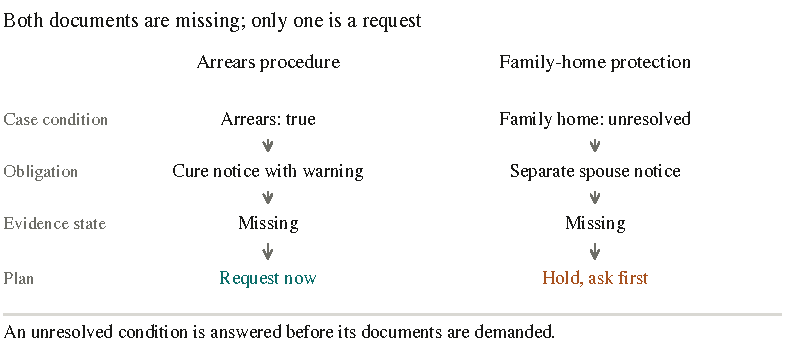
\includegraphics[width=.85\linewidth]{fig_native_case.pdf}
\caption{\textbf{A recorded controller decision.} In the first completed
\casepath development case in sorted cohort order, arrears is true and
family-home status unresolved. The cure notice is requested now; the spouse
notice remains conditional. This shows two routes within the recorded plan,
not an accepted native graph: its exported predicate namespace encounters the
same interface failure as the other generated artefacts. The release includes
the complete case trace and selection rule.}
\label{fig:native-case}
\end{figure}

\paragraph{Execution evidence and historical access.}
The primary scoring task authenticates both complete prediction inventories
before reading references. The original producer terminated without its
complete I/O audit; historical non-access to protected targets is therefore
not established retrospectively. Scoring, the compatibility diagnosis and
the request-only analysis are separately recorded, with original failures
preserved. All original target containers are subsequently released as exact
bytes under their recorded data license. This version is now a public
benchmark and cannot serve as newly hidden confirmation.

\paragraph{Offline reproduction.}
The anonymous artifact contains all \nbCells{} prediction and failure cells,
the exact \nbClaims{} reference containers, original native evaluator,
reporting code, source commitments and request-only wrapper. Network-disabled
replay reproduces both primary phase reports, the complete primary report,
every request-only row and its descriptive report by exact canonical JSON
comparison, without a numerical tolerance. This reproduces scoring from
recorded model outputs; it does not regenerate those outputs or provide the
remote model checkpoint.

\end{document}
